%%
% Copyright (c) 2017 - 2023, Pascal Wagler;
% Copyright (c) 2014 - 2023, John MacFarlane
%
% All rights reserved.
%
% Redistribution and use in source and binary forms, with or without
% modification, are permitted provided that the following conditions
% are met:
%
% - Redistributions of source code must retain the above copyright
% notice, this list of conditions and the following disclaimer.
%
% - Redistributions in binary form must reproduce the above copyright
% notice, this list of conditions and the following disclaimer in the
% documentation and/or other materials provided with the distribution.
%
% - Neither the name of John MacFarlane nor the names of other
% contributors may be used to endorse or promote products derived
% from this software without specific prior written permission.
%
% THIS SOFTWARE IS PROVIDED BY THE COPYRIGHT HOLDERS AND CONTRIBUTORS
% "AS IS" AND ANY EXPRESS OR IMPLIED WARRANTIES, INCLUDING, BUT NOT
% LIMITED TO, THE IMPLIED WARRANTIES OF MERCHANTABILITY AND FITNESS
% FOR A PARTICULAR PURPOSE ARE DISCLAIMED. IN NO EVENT SHALL THE
% COPYRIGHT OWNER OR CONTRIBUTORS BE LIABLE FOR ANY DIRECT, INDIRECT,
% INCIDENTAL, SPECIAL, EXEMPLARY, OR CONSEQUENTIAL DAMAGES (INCLUDING,
% BUT NOT LIMITED TO, PROCUREMENT OF SUBSTITUTE GOODS OR SERVICES;
% LOSS OF USE, DATA, OR PROFITS; OR BUSINESS INTERRUPTION) HOWEVER
% CAUSED AND ON ANY THEORY OF LIABILITY, WHETHER IN CONTRACT, STRICT
% LIABILITY, OR TORT (INCLUDING NEGLIGENCE OR OTHERWISE) ARISING IN
% ANY WAY OUT OF THE USE OF THIS SOFTWARE, EVEN IF ADVISED OF THE
% POSSIBILITY OF SUCH DAMAGE.
%%

%%
% This is the Eisvogel pandoc LaTeX template.
%
% For usage information and examples visit the official GitHub page:
% https://github.com/Wandmalfarbe/pandoc-latex-template
%%

% Options for packages loaded elsewhere
\PassOptionsToPackage{unicode,linktoc=all}{hyperref}
\PassOptionsToPackage{hyphens}{url}
\PassOptionsToPackage{dvipsnames,svgnames,x11names,table}{xcolor}


%
\documentclass[
  10pt,
  paper=a4,
  ,captions=tableheading
]{scrartcl}
\usepackage{amsmath,amssymb}
% Use setspace anyway because we change the default line spacing.
% The spacing is changed early to affect the titlepage and the TOC.
\usepackage{setspace}
\setstretch{1.2}
\usepackage{iftex}
\ifPDFTeX
  \usepackage[T1]{fontenc}
  \usepackage[utf8]{inputenc}
  \usepackage{textcomp} % provide euro and other symbols
\else % if luatex or xetex
  \usepackage{unicode-math} % this also loads fontspec
  \defaultfontfeatures{Scale=MatchLowercase}
  \defaultfontfeatures[\rmfamily]{Ligatures=TeX,Scale=1}
\fi
\usepackage{lmodern}
\ifPDFTeX\else
  % xetex/luatex font selection
\fi
% Use upquote if available, for straight quotes in verbatim environments
\IfFileExists{upquote.sty}{\usepackage{upquote}}{}
\IfFileExists{microtype.sty}{% use microtype if available
  \usepackage[]{microtype}
  \UseMicrotypeSet[protrusion]{basicmath} % disable protrusion for tt fonts
}{}
\makeatletter
\@ifundefined{KOMAClassName}{% if non-KOMA class
  \IfFileExists{parskip.sty}{%
    \usepackage{parskip}
  }{% else
    \setlength{\parindent}{0pt}
    \setlength{\parskip}{6pt plus 2pt minus 1pt}}
}{% if KOMA class
  \KOMAoptions{parskip=half}}
\makeatother
\usepackage{xcolor}
\definecolor{UniPDColor}{RGB}{155, 0, 20}
\definecolor{default-linkcolor}{RGB}{155, 0, 20}
\definecolor{default-filecolor}{RGB}{155, 0, 20}
\definecolor{default-citecolor}{RGB}{155, 0, 20}
\definecolor{default-urlcolor}{HTML}{4077C0}
\usepackage[margin=2.0cm,includehead=true,includefoot=true,centering,]{geometry}
\usepackage{color}
\usepackage{fancyvrb}
\newcommand{\VerbBar}{|}
\newcommand{\VERB}{\Verb[commandchars=\\\{\}]}
\DefineVerbatimEnvironment{Highlighting}{Verbatim}{commandchars=\\\{\}}
% Add ',fontsize=\small' for more characters per line
\usepackage{framed}
\definecolor{shadecolor}{RGB}{248,248,248}
\newenvironment{Shaded}{\begin{snugshade}}{\end{snugshade}}
\newcommand{\AlertTok}[1]{\textcolor[rgb]{0.94,0.16,0.16}{#1}}
\newcommand{\AnnotationTok}[1]{\textcolor[rgb]{0.56,0.35,0.01}{\textbf{\textit{#1}}}}
\newcommand{\AttributeTok}[1]{\textcolor[rgb]{0.13,0.29,0.53}{#1}}
\newcommand{\BaseNTok}[1]{\textcolor[rgb]{0.00,0.00,0.81}{#1}}
\newcommand{\BuiltInTok}[1]{#1}
\newcommand{\CharTok}[1]{\textcolor[rgb]{0.31,0.60,0.02}{#1}}
\newcommand{\CommentTok}[1]{\textcolor[rgb]{0.56,0.35,0.01}{\textit{#1}}}
\newcommand{\CommentVarTok}[1]{\textcolor[rgb]{0.56,0.35,0.01}{\textbf{\textit{#1}}}}
\newcommand{\ConstantTok}[1]{\textcolor[rgb]{0.56,0.35,0.01}{#1}}
\newcommand{\ControlFlowTok}[1]{\textcolor[rgb]{0.13,0.29,0.53}{\textbf{#1}}}
\newcommand{\DataTypeTok}[1]{\textcolor[rgb]{0.13,0.29,0.53}{#1}}
\newcommand{\DecValTok}[1]{\textcolor[rgb]{0.00,0.00,0.81}{#1}}
\newcommand{\DocumentationTok}[1]{\textcolor[rgb]{0.56,0.35,0.01}{\textbf{\textit{#1}}}}
\newcommand{\ErrorTok}[1]{\textcolor[rgb]{0.64,0.00,0.00}{\textbf{#1}}}
\newcommand{\ExtensionTok}[1]{#1}
\newcommand{\FloatTok}[1]{\textcolor[rgb]{0.00,0.00,0.81}{#1}}
\newcommand{\FunctionTok}[1]{\textcolor[rgb]{0.13,0.29,0.53}{\textbf{#1}}}
\newcommand{\ImportTok}[1]{#1}
\newcommand{\InformationTok}[1]{\textcolor[rgb]{0.56,0.35,0.01}{\textbf{\textit{#1}}}}
\newcommand{\KeywordTok}[1]{\textcolor[rgb]{0.13,0.29,0.53}{\textbf{#1}}}
\newcommand{\NormalTok}[1]{#1}
\newcommand{\OperatorTok}[1]{\textcolor[rgb]{0.81,0.36,0.00}{\textbf{#1}}}
\newcommand{\OtherTok}[1]{\textcolor[rgb]{0.56,0.35,0.01}{#1}}
\newcommand{\PreprocessorTok}[1]{\textcolor[rgb]{0.56,0.35,0.01}{\textit{#1}}}
\newcommand{\RegionMarkerTok}[1]{#1}
\newcommand{\SpecialCharTok}[1]{\textcolor[rgb]{0.81,0.36,0.00}{\textbf{#1}}}
\newcommand{\SpecialStringTok}[1]{\textcolor[rgb]{0.31,0.60,0.02}{#1}}
\newcommand{\StringTok}[1]{\textcolor[rgb]{0.31,0.60,0.02}{#1}}
\newcommand{\VariableTok}[1]{\textcolor[rgb]{0.00,0.00,0.00}{#1}}
\newcommand{\VerbatimStringTok}[1]{\textcolor[rgb]{0.31,0.60,0.02}{#1}}
\newcommand{\WarningTok}[1]{\textcolor[rgb]{0.56,0.35,0.01}{\textbf{\textit{#1}}}}

% Workaround/bugfix from jannick0.
% See https://github.com/jgm/pandoc/issues/4302#issuecomment-360669013)
% or https://github.com/Wandmalfarbe/pandoc-latex-template/issues/2
%
% Redefine the verbatim environment 'Highlighting' to break long lines (with
% the help of fvextra). Redefinition is necessary because it is unlikely that
% pandoc includes fvextra in the default template.
\usepackage{fvextra}
\DefineVerbatimEnvironment{Highlighting}{Verbatim}{breaklines,fontsize=\small,commandchars=\\\{\}}

\usepackage{longtable,booktabs,array}
\usepackage{calc} % for calculating minipage widths
% Correct order of tables after \paragraph or \subparagraph
\usepackage{etoolbox}
\makeatletter
\patchcmd\longtable{\par}{\if@noskipsec\mbox{}\fi\par}{}{}
\makeatother
% Allow footnotes in longtable head/foot
\IfFileExists{footnotehyper.sty}{\usepackage{footnotehyper}}{\usepackage{footnote}}
\makesavenoteenv{longtable}
% add backlinks to footnote references, cf. https://tex.stackexchange.com/questions/302266/make-footnote-clickable-both-ways
\usepackage{footnotebackref}
\usepackage{graphicx}
\makeatletter
\def\maxwidth{\ifdim\Gin@nat@width>\linewidth\linewidth\else\Gin@nat@width\fi}
\def\maxheight{\ifdim\Gin@nat@height>\textheight\textheight\else\Gin@nat@height\fi}
\makeatother
% Scale images if necessary, so that they will not overflow the page
% margins by default, and it is still possible to overwrite the defaults
% using explicit options in \includegraphics[width, height, ...]{}
\setkeys{Gin}{width=\maxwidth,height=\maxheight,keepaspectratio}
% Set default figure placement to htbp
\makeatletter
% Make use of float-package and set default placement for figures to H.
% The option H means 'PUT IT HERE' (as  opposed to the standard h option which means 'You may put it here if you like').
\usepackage{float}
\floatplacement{figure}{H}
\makeatother
\setlength{\emergencystretch}{3em} % prevent overfull lines
\providecommand{\tightlist}{%
  \setlength{\itemsep}{0pt}\setlength{\parskip}{0pt}}
\setcounter{secnumdepth}{-\maxdimen} % remove section numbering
\ifLuaTeX
\usepackage[bidi=basic]{babel}
\else
\usepackage[bidi=default]{babel}
\fi
\babelprovide[main,import]{british}
% get rid of language-specific shorthands (see #6817):
\let\LanguageShortHands\languageshorthands
\def\languageshorthands#1{}
\usepackage{setspace}
\newpage
\usepackage{hyperref}
\usepackage{multirow}
\usepackage{amsmath}
\usepackage{algorithm}
\usepackage{algorithmic}
\usepackage{authblk}
\usepackage{graphicx}
\usepackage{fancyvrb}
\RecustomVerbatimEnvironment{Verbatim}{BVerbatim}{breaklines=true,breakanywhere=true}
\ifLuaTeX
  \usepackage{selnolig}  % disable illegal ligatures
\fi
\usepackage[]{natbib}
\bibliographystyle{apsr}
\usepackage[strings]{underscore} % protect underscores in most circumstances
\IfFileExists{bookmark.sty}{\usepackage{bookmark}}{\usepackage{hyperref}}
\IfFileExists{xurl.sty}{\usepackage{xurl}}{} % add URL line breaks if available
\urlstyle{same}
\hypersetup{
  pdftitle={Statistical Learning Final Project},
  pdfauthor={Zeynep TUTAR - 2106038; Aysenur Oya ÖZEN - 2107501},
  pdflang={en-GB},
  colorlinks=true,
  linkcolor={default-linkcolor},
  filecolor={default-filecolor},
  citecolor={default-citecolor},
  urlcolor={default-urlcolor},
  breaklinks=true,
  pdfcreator={LaTeX via pandoc with the Eisvogel template}}
\title{Statistical Learning Final Project}
\usepackage{etoolbox}
\makeatletter
\providecommand{\subtitle}[1]{% add subtitle to \maketitle
  \apptocmd{\@title}{\par {\large #1 \par}}{}{}
}
\makeatother
\subtitle{Employee Attrition Classification}
\author{Zeynep TUTAR - 2106038 \and Aysenur Oya ÖZEN - 2107501}
\date{09-07-2024}



%%
%% added
%%

\usepackage{silence}
\WarningsOff[everypage]% Suppress warnings related to package everypage


%
% for the background color of the title page
%
\usepackage{pagecolor}
\usepackage{afterpage}
\usepackage{tikz}
\usepackage[margin=2.0cm,includehead=true,includefoot=true,centering]{geometry}

%
% break urls
%
\PassOptionsToPackage{hyphens}{url}

%
% When using babel or polyglossia with biblatex, loading csquotes is recommended
% to ensure that quoted texts are typeset according to the rules of your main language.
%
\usepackage{csquotes}

%
% captions
%
\definecolor{caption-color}{RGB}{155, 0, 20}
%{HTML}{777777}
\usepackage[font={stretch=1.2}, textfont={color=caption-color}, position=top, skip=4mm, labelfont=bf, singlelinecheck=false, justification=raggedright]{caption}
\setcapindent{0em}

%
% blockquote
%
\definecolor{blockquote-border}{RGB}{155, 0, 20}
\definecolor{blockquote-text}{RGB}{155, 0, 20}
\usepackage{mdframed}
\newmdenv[rightline=false,bottomline=false,topline=false,linewidth=3pt,linecolor=blockquote-border,skipabove=\parskip]{customblockquote}
\renewenvironment{quote}{\begin{customblockquote}\list{}{\rightmargin=0em\leftmargin=0em}%
\item\relax\color{blockquote-text}\ignorespaces}{\unskip\unskip\endlist\end{customblockquote}}

%
% Source Sans Pro as the default font family
% Source Code Pro for monospace text
%
% 'default' option sets the default
% font family to Source Sans Pro, not \sfdefault.
%
\ifnum 0\ifxetex 1\fi\ifluatex 1\fi=0 % if pdftex
    %\usepackage[default]{sourcesanspro}
  \usepackage{sourcecodepro}
  \else % if not pdftex
    \usepackage[default]{sourcesanspro}
  \usepackage{sourcecodepro}

  % XeLaTeX specific adjustments for straight quotes: https://tex.stackexchange.com/a/354887
  % This issue is already fixed (see https://github.com/silkeh/latex-sourcecodepro/pull/5) but the
  % fix is still unreleased.
  % TODO: Remove this workaround when the new version of sourcecodepro is released on CTAN.
  \ifxetex
    \makeatletter
    \defaultfontfeatures[\ttfamily]
      { Numbers   = \sourcecodepro@figurestyle,
        Scale     = \SourceCodePro@scale,
        Extension = .otf }
    \setmonofont
      [ UprightFont    = *-\sourcecodepro@regstyle,
        ItalicFont     = *-\sourcecodepro@regstyle It,
        BoldFont       = *-\sourcecodepro@boldstyle,
        BoldItalicFont = *-\sourcecodepro@boldstyle It ]
      {SourceCodePro}
    \makeatother
  \fi
  \fi

%
% heading color
%
\definecolor{heading-color}{RGB}{40,40,40}
\addtokomafont{section}{\color{heading-color}}
% When using the classes report, scrreprt, book,
% scrbook or memoir, uncomment the following line.
%\addtokomafont{chapter}{\color{heading-color}}

%
% variables for title, author and date
%
\usepackage{titling}
\title{Statistical Learning Final Project}
\author{Zeynep TUTAR - 2106038, Aysenur Oya ÖZEN - 2107501}
\date{09-07-2024}

%
% tables
%

\definecolor{table-row-color}{HTML}{F5F5F5}
\definecolor{table-rule-color}{HTML}{999999}

%\arrayrulecolor{black!40}
\arrayrulecolor{table-rule-color}     % color of \toprule, \midrule, \bottomrule
\setlength\heavyrulewidth{0.3ex}      % thickness of \toprule, \bottomrule
\renewcommand{\arraystretch}{1.3}     % spacing (padding)


%
% remove paragraph indentation
%
\setlength{\parindent}{0pt}
\setlength{\parskip}{6pt plus 2pt minus 1pt}
\setlength{\emergencystretch}{3em}  % prevent overfull lines

%
%
% Listings
%
%


%
% header and footer
%

\definecolor{headfoot-color}{RGB}{134, 134, 134}
\usepackage[headsepline,footsepline]{scrlayer-scrpage}

\newpairofpagestyles{eisvogel-header-footer}{
  \clearpairofpagestyles
  \ihead*{\color{headfoot-color}Employee Attrition Classification}
  \chead*{\color{headfoot-color}\leftmark}
  \ohead*{\color{headfoot-color}\thetitle}
  \ifoot*{\color{headfoot-color}\hspace{1cm}}
  \cfoot*{\color{headfoot-color}Page \thepage}
  \ofoot*{\color{headfoot-color}\hspace{1cm}}
  \addtokomafont{pageheadfoot}{\upshape}
  \addtokomafont{headsepline}{\color{headfoot-color}}
  \addtokomafont{footsepline}{\color{headfoot-color}}
}
\pagestyle{eisvogel-header-footer}



%%
%% end added
%%

\begin{document}

%%
%% begin titlepage
%%
\begin{titlepage}
\newgeometry{top=2cm, right=3cm, bottom=3cm, left=3cm}
\tikz[remember picture,overlay] \node[inner sep=0pt] at (current page.center){\vspace{-5cm}{
\includegraphics[width=27cm, height=27cm]{img/unipdbg.pdf}}};
%\newcommand{\colorRule}[3][black]{\textcolor[HTML]{#1}{\rule{#2}{#3}}}
\begin{center}
\noindent
\\[-1em]
\color[HTML]{5F5F5F}
%\makebox[0pt][l]{\colorRule[435488]{1.3\textwidth}{4pt}}
\par
\noindent

% The titlepage with a background image has other text spacing and text size
{
  \vspace{-2cm}
  
\includegraphics[height=2.25cm]{img/logo-unipd.pdf}
  \hfill
  
\includegraphics[height=1.75cm]{img/logo-long-mat.png}
  \par
  \vspace{0.5cm}
  \mbox{}\\[2.0cm]
  \null \vspace{\stretch{2}}
  \Large\textsc{Statistical Learning Final Project} \\

  % title
  \vspace{3ex}
  \Huge\textbf{\color{UniPDColor}Employee Attrition Classification} \\
  \vspace{\stretch{2.5}}

  % authors, advisors etc...
  \normalsize
  \textsc{Authors} \\
  \Large{\textbf{Zeynep TUTAR - 2106038 \\
      Aysenur Oya ÖZEN - 2107501}} \\
  \vspace{\stretch{1}} \null
  \normalsize
  \textsc{Supervisor} \\
  \Large{\textbf{Prof. Alberto ROVERATO}} \\
  
  \vspace{\stretch{1}} \null
  \Large{\textbf{Academic Year: \\2023/2024}}
}


\end{center}
\end{titlepage}
\restoregeometry
\pagenumbering{arabic}

%%
%% end titlepage
%%

% \maketitle


{
\hypersetup{linkcolor=}
\setcounter{tocdepth}{3}
\tableofcontents
\newpage
}
\section{Introduction to Dataset}\label{introduction-to-dataset}

The aim of this project is to develop two predictive models to determine
employee attrition of a company. The dataset\footnote{\url{https://www.kaggle.com/datasets/stealthtechnologies/employee-attrition-dataset/data}}
used for this project is a simulated dataset designed for the analysis
and prediction of employee attrition. It contains detailed information
about various aspects of an employee's profile, including demographics,
job-related features, and personal circumstances.The dataset contains
74,498 samples. Each record includes a unique Employee ID and features
that influence employee attrition. The goal is to understand the factors
contributing to attrition and develop predictive models to identify
at-risk employees.

The dataset is already split into train and test but in order to better
understand the data, it is crucial to analyse the dataset as a whole.

\small

\begin{Shaded}
\begin{Highlighting}[]
\CommentTok{\# import the train and test datasets}
\NormalTok{data\_train }\OtherTok{\textless{}{-}} \FunctionTok{read.csv}\NormalTok{(}\StringTok{"data/train.csv"}\NormalTok{, }\AttributeTok{stringsAsFactors =} \ConstantTok{TRUE}\NormalTok{)}
\NormalTok{data\_test }\OtherTok{\textless{}{-}} \FunctionTok{read.csv}\NormalTok{(}\StringTok{"data/test.csv"}\NormalTok{, }\AttributeTok{stringsAsFactors =} \ConstantTok{TRUE}\NormalTok{)}

\CommentTok{\# merge the datasets}
\NormalTok{data }\OtherTok{\textless{}{-}} \FunctionTok{rbind}\NormalTok{(data\_train, data\_test)}
\FunctionTok{attach}\NormalTok{(data)}
\end{Highlighting}
\end{Shaded}

\small

\subsection{Description of the
Features}\label{description-of-the-features}

The features of the dataset are presented below:

\begin{itemize}
\item
  \textbf{Employee ID:} A unique identifier assigned to each employee.
\item
  \textbf{Age:} The age of the employee, ranging from 18 to 60 years.
\item
  \textbf{Gender:} The gender of the employee
\item
  \textbf{Years at Company:} The number of years the employee has been
  working at the company.
\item
  \textbf{Monthly Income:} The monthly salary of the employee, in
  dollars.
\item
  \textbf{Job Role:} The department or role the employee works in,
  encoded into categories such as Finance, Healthcare, Technology,
  Education, and Media.
\item
  \textbf{Work-Life Balance:} The employee's perceived balance between
  work and personal life
\item
  \textbf{Job Satisfaction:} The employee's satisfaction with their job
\item
  \textbf{Performance Rating:} The employee's performance rating
\item
  \textbf{Number of Promotions:} The total number of promotions the
  employee has received.
\item
  \textbf{Distance from Home:} The distance between the employee's home
  and workplace, in miles.
\item
  \textbf{Education Level:} The highest education level attained by the
  employee
\item
  \textbf{Marital Status:} The marital status of the employee
\item
  \textbf{Job Level:} The job level of the employee
\item
  \textbf{Company Size:} The size of the company the employee works for
\item
  \textbf{Company Tenure:} The total number of years the employee has
  been working in the industry.
\item
  \textbf{Remote Work:} Whether the employee works remotely
\item
  \textbf{Leadership Opportunities:} Whether the employee has leadership
  opportunities
\item
  \textbf{Innovation Opportunities:} Whether the employee has
  opportunities for innovation
\item
  \textbf{Company Reputation:} The employee's perception of the
  company's reputation
\item
  \textbf{Employee Recognition:} The level of recognition the employee
  receives
\item
  \textbf{Attrition:} Whether the employee has left the company
\end{itemize}

\section{Data Analysis}\label{data-analysis}

In order to develop predictive models, first it is necessary to perform
exploratory data analysis (EDA) and modify the format of the data if
necessary.

\small

\begin{Shaded}
\begin{Highlighting}[]
\CommentTok{\# installing required libraries}
\FunctionTok{library}\NormalTok{(class)}
\FunctionTok{library}\NormalTok{(car)}
\FunctionTok{library}\NormalTok{(corrplot)}
\FunctionTok{library}\NormalTok{(glmnet)}
\FunctionTok{library}\NormalTok{(pROC)}
\FunctionTok{library}\NormalTok{(knitr)}
\FunctionTok{library}\NormalTok{(leaps)}
\FunctionTok{library}\NormalTok{(MASS)}
\end{Highlighting}
\end{Shaded}

\small

\small

\begin{Shaded}
\begin{Highlighting}[]
\CommentTok{\# Descriptive statistics}
\FunctionTok{str}\NormalTok{(data)}
\end{Highlighting}
\end{Shaded}

\begin{verbatim}
'data.frame':   74498 obs. of  24 variables:
 $ Employee.ID             : int  8410 64756 30257 65791 65026 24368 64970 36999 32714 15944 ...
 $ Age                     : int  31 59 24 36 56 38 47 48 57 24 ...
 $ Gender                  : Factor w/ 2 levels "Female","Male": 2 1 1 1 2 1 2 2 2 1 ...
 $ Years.at.Company        : int  19 4 10 7 41 3 23 16 44 1 ...
 $ Job.Role                : Factor w/ 5 levels "Education","Finance",..: 1 4 3 1 1 5 1 2 1 3 ...
 $ Monthly.Income          : int  5390 5534 8159 3989 4821 9977 3681 11223 3773 7319 ...
 $ Work.Life.Balance       : Factor w/ 4 levels "Excellent","Fair",..: 1 4 3 3 2 2 2 1 3 4 ...
 $ Job.Satisfaction        : Factor w/ 4 levels "High","Low","Medium",..: 3 1 1 1 4 1 1 4 3 1 ...
 $ Performance.Rating      : Factor w/ 4 levels "Average","Below Average",..: 1 4 4 3 1 2 3 3 3 1 ...
 $ Number.of.Promotions    : int  2 3 0 1 0 3 1 2 1 1 ...
 $ Overtime                : Factor w/ 2 levels "No","Yes": 1 1 1 1 2 1 2 1 2 2 ...
 $ Distance.from.Home      : int  22 21 11 27 71 37 75 5 39 57 ...
 $ Education.Level         : Factor w/ 5 levels "Associate Degree",..: 1 4 2 3 3 2 3 4 3 5 ...
 $ Marital.Status          : Factor w/ 3 levels "Divorced","Married",..: 2 1 2 3 1 2 1 2 2 3 ...
 $ Number.of.Dependents    : int  0 3 3 2 0 0 3 4 4 4 ...
 $ Job.Level               : Factor w/ 3 levels "Entry","Mid",..: 2 2 2 2 3 2 1 1 1 1 ...
 $ Company.Size            : Factor w/ 3 levels "Large","Medium",..: 2 2 2 3 2 2 3 2 2 1 ...
 $ Company.Tenure          : int  89 21 74 50 68 47 93 88 75 45 ...
 $ Remote.Work             : Factor w/ 2 levels "No","Yes": 1 1 1 2 1 1 1 1 1 1 ...
 $ Leadership.Opportunities: Factor w/ 2 levels "No","Yes": 1 1 1 1 1 1 1 1 1 1 ...
 $ Innovation.Opportunities: Factor w/ 2 levels "No","Yes": 1 1 1 1 1 2 1 1 1 2 ...
 $ Company.Reputation      : Factor w/ 4 levels "Excellent","Fair",..: 1 2 4 3 2 2 3 1 2 3 ...
 $ Employee.Recognition    : Factor w/ 4 levels "High","Low","Medium",..: 3 2 2 3 3 1 3 2 3 2 ...
 $ Attrition               : Factor w/ 2 levels "Left","Stayed": 2 2 2 2 2 1 1 2 2 1 ...
\end{verbatim}

\small

\subsection{Data Preprocessing}\label{data-preprocessing}

To prepare the dataset for further analysis, several data preprocessing
steps are performed:

\begin{enumerate}
\def\labelenumi{\arabic{enumi}.}
\tightlist
\item
  Removing Columns
\end{enumerate}

Employee.ID and Company.Tenure dropped as they are not useful for
predictive modeling. Company.Tenure column gives logically incorrect
numerical values.

\small

\begin{Shaded}
\begin{Highlighting}[]
\CommentTok{\# Drop Employee Id and Company.Tenure}
\NormalTok{data }\OtherTok{\textless{}{-}}\NormalTok{ data[, }\SpecialCharTok{!}\FunctionTok{names}\NormalTok{(data) }\SpecialCharTok{\%in\%} \StringTok{"Employee.ID"}\NormalTok{]}
\NormalTok{data }\OtherTok{\textless{}{-}}\NormalTok{ data[, }\SpecialCharTok{!}\FunctionTok{names}\NormalTok{(data) }\SpecialCharTok{\%in\%} \StringTok{"Company.Tenure"}\NormalTok{]}

\CommentTok{\# Copy Data for further Analysis}
\NormalTok{data\_detailed }\OtherTok{\textless{}{-}}\NormalTok{ data}
\end{Highlighting}
\end{Shaded}

\small

\begin{enumerate}
\def\labelenumi{\arabic{enumi}.}
\setcounter{enumi}{1}
\tightlist
\item
  Numerical and Categorical Variables Separation
\end{enumerate}

Numerical and categorical variables were separated for targeted
analysis. Summary statistics were then used to provide a quick overview
of the distribution of numerical features.

Summary statistics for numerical variables reveal that the ages of
employees range from 18 to 59,indicating a workforce that spans multiple
generations.Employees have been with the company for a wide range of 1
to 51 years suggesting a mix of new and long-term staff.Monthly incomes
vary widely, from 1,226 to 16,149 units, indicating financial situation
specific to the individual, industry or other variables. Lastly, the
distance from home ranges from 1 to 99 units, which suggests that while
some employees live close to their workplace, others may have longer
commutes. This variability highlights the diverse nature of the
workforce.

\small

\begin{Shaded}
\begin{Highlighting}[]
\CommentTok{\# Numerical and categorical variables separation}
\NormalTok{numeric\_vars }\OtherTok{\textless{}{-}} \FunctionTok{sapply}\NormalTok{(data, is.numeric)}
\NormalTok{categoric\_vars }\OtherTok{\textless{}{-}} \FunctionTok{sapply}\NormalTok{(data, }\ControlFlowTok{function}\NormalTok{(x) }\FunctionTok{is.factor}\NormalTok{(x) }\SpecialCharTok{||} \FunctionTok{is.character}\NormalTok{(x))}

\CommentTok{\# Taking names from numerical and categorical variables for}
\CommentTok{\# distribution graph}
\NormalTok{categoric\_var\_names }\OtherTok{\textless{}{-}} \FunctionTok{names}\NormalTok{(data)[categoric\_vars]}
\NormalTok{numeric\_var\_names }\OtherTok{\textless{}{-}} \FunctionTok{names}\NormalTok{(data)[numeric\_vars]}

\CommentTok{\# Numeric values summary}
\FunctionTok{summary}\NormalTok{(data[, numeric\_vars])}
\end{Highlighting}
\end{Shaded}

\begin{verbatim}
      Age        Years.at.Company Monthly.Income  Number.of.Promotions
 Min.   :18.00   Min.   : 1.00    Min.   : 1226   Min.   :0.0000      
 1st Qu.:28.00   1st Qu.: 7.00    1st Qu.: 5652   1st Qu.:0.0000      
 Median :39.00   Median :13.00    Median : 7348   Median :1.0000      
 Mean   :38.53   Mean   :15.72    Mean   : 7299   Mean   :0.8329      
 3rd Qu.:49.00   3rd Qu.:23.00    3rd Qu.: 8876   3rd Qu.:2.0000      
 Max.   :59.00   Max.   :51.00    Max.   :16149   Max.   :4.0000      
 Distance.from.Home Number.of.Dependents
 Min.   : 1.00      Min.   :0.00        
 1st Qu.:25.00      1st Qu.:0.00        
 Median :50.00      Median :1.00        
 Mean   :49.99      Mean   :1.65        
 3rd Qu.:75.00      3rd Qu.:3.00        
 Max.   :99.00      Max.   :6.00        
\end{verbatim}

\small

\begin{enumerate}
\def\labelenumi{\arabic{enumi}.}
\setcounter{enumi}{2}
\tightlist
\item
  Missing Values Analysis
\end{enumerate}

No missing values were found in the data set, so there was no need to
apply removing of null values operation.

\small

\begin{Shaded}
\begin{Highlighting}[]
\CommentTok{\# Checking if there are missing values in the entire dataset}
\NormalTok{total\_na }\OtherTok{\textless{}{-}} \FunctionTok{sum}\NormalTok{(}\FunctionTok{is.na}\NormalTok{(data))}
\FunctionTok{cat}\NormalTok{(}\StringTok{"Total number of missing values:"}\NormalTok{, total\_na, }\StringTok{"}\SpecialCharTok{\textbackslash{}n}\StringTok{"}\NormalTok{)}
\end{Highlighting}
\end{Shaded}

\begin{verbatim}
Total number of missing values: 0 
\end{verbatim}

\small

\begin{enumerate}
\def\labelenumi{\arabic{enumi}.}
\setcounter{enumi}{3}
\tightlist
\item
  Categorical Variables Distribution
\end{enumerate}

Inferences from the bar charts of categorical variables: The fact that
the gender distribution is almost equal shows that there is no gender
bias in the data.Job roles skew towards technology and media, indicating
a focus on these sectors.Most employees rate their work-life balance as
good or excellent; This indicates high satisfaction; however, job
satisfaction varies, with some rating it as low or medium.Performance
ratings are mostly average, indicating a need for better performance
management.The fact that most employees have not received any promotions
highlights potential career development issues.Overtime is rare,
indicating manageable workloads.Education levels vary, and many have
bachelor's degrees.Marital status indicates more married workers.Job
levels are mostly entry and intermediate, indicating a younger
workforce.Company size is evenly distributed, indicating different
operational scales.The rarity of remote work points to traditional
office culture.Limited leadership and innovation opportunities suggest
areas for development.The company's reputation is mostly good, but
employee recognition is low to moderate, indicating room for
improvement.

\small

\begin{Shaded}
\begin{Highlighting}[]
\CommentTok{\# Categorical variables distribution}
\FunctionTok{par}\NormalTok{(}\AttributeTok{mfrow =} \FunctionTok{c}\NormalTok{(}\DecValTok{3}\NormalTok{, }\DecValTok{5}\NormalTok{), }\AttributeTok{mar =} \FunctionTok{c}\NormalTok{(}\DecValTok{5}\NormalTok{, }\DecValTok{4}\NormalTok{, }\DecValTok{2}\NormalTok{, }\DecValTok{2}\NormalTok{) }\SpecialCharTok{+} \FloatTok{0.1}\NormalTok{)}
\ControlFlowTok{for}\NormalTok{ (cat\_var }\ControlFlowTok{in}\NormalTok{ categoric\_var\_names[}\SpecialCharTok{{-}}\DecValTok{16}\NormalTok{]) \{}
    \FunctionTok{barplot}\NormalTok{(}\FunctionTok{table}\NormalTok{(data[[cat\_var]]), }\AttributeTok{main =} \FunctionTok{paste}\NormalTok{(cat\_var), }\AttributeTok{ylab =} \StringTok{"Count"}\NormalTok{,}
        \AttributeTok{col =} \StringTok{"firebrick4"}\NormalTok{, }\AttributeTok{cex.names =} \FloatTok{0.7}\NormalTok{, }\AttributeTok{las =} \DecValTok{2}\NormalTok{, }\AttributeTok{cex.main =} \FloatTok{0.9}\NormalTok{, }\AttributeTok{cex.axis =} \FloatTok{0.8}\NormalTok{)}
\NormalTok{\}}
\end{Highlighting}
\end{Shaded}

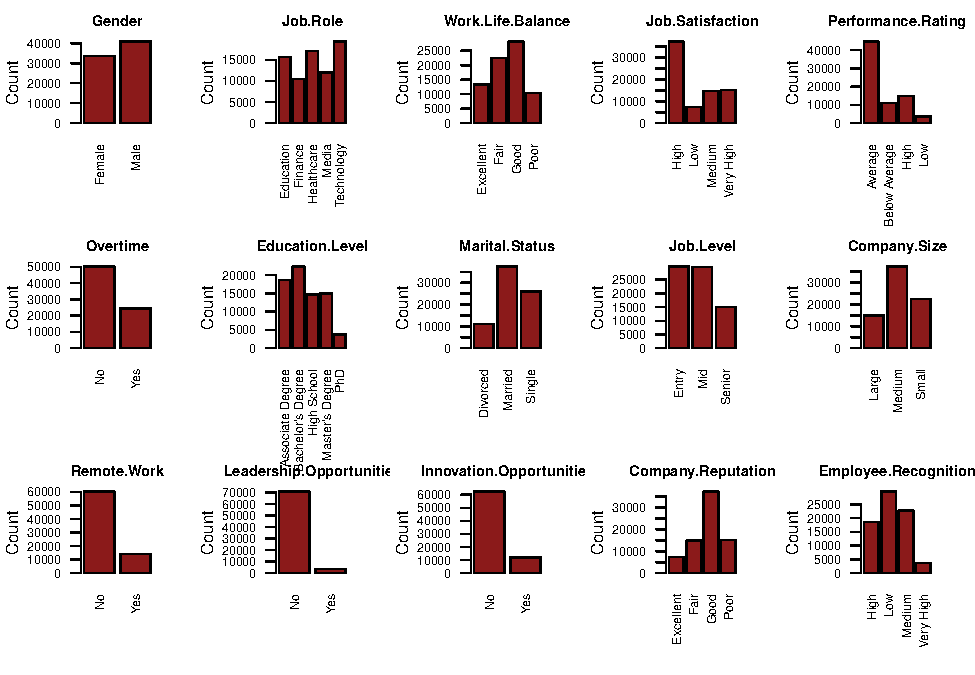
\includegraphics{figs/data_catdist-1.pdf}

\small

\begin{enumerate}
\def\labelenumi{\arabic{enumi}.}
\setcounter{enumi}{4}
\tightlist
\item
  Numerical Values Distribution
\end{enumerate}

Inferences from the histograms for the numerical variables: The age
distribution is fairly uniform, indicating a wide age range among
employees.The years at the company show a right-skewed distribution,
with most employees having shorter tenures and fewer employees staying
beyond 30 years.Monthly income has a roughly normal distribution,
peaking around 5,000 to 10,000 units, suggesting that most employees
earn within this range.The distance from home distribution is relatively
uniform, indicating that employees live at various distances from their
workplace.

\small

\begin{Shaded}
\begin{Highlighting}[]
\CommentTok{\# Numerical variables distribution}
\FunctionTok{par}\NormalTok{(}\AttributeTok{mfrow =} \FunctionTok{c}\NormalTok{(}\DecValTok{2}\NormalTok{, }\DecValTok{3}\NormalTok{), }\AttributeTok{mar =} \FunctionTok{c}\NormalTok{(}\DecValTok{3}\NormalTok{, }\DecValTok{3}\NormalTok{, }\DecValTok{2}\NormalTok{, }\DecValTok{1}\NormalTok{))}
\ControlFlowTok{for}\NormalTok{ (num\_var }\ControlFlowTok{in}\NormalTok{ numeric\_var\_names) \{}
    \FunctionTok{hist}\NormalTok{(data[[num\_var]], }\AttributeTok{main =} \FunctionTok{paste}\NormalTok{(num\_var), }\AttributeTok{xlab =} \StringTok{""}\NormalTok{, }\AttributeTok{ylab =} \StringTok{""}\NormalTok{, }\AttributeTok{col =} \StringTok{"firebrick4"}\NormalTok{,}
        \AttributeTok{breaks =} \DecValTok{30}\NormalTok{, }\AttributeTok{cex.main =} \FloatTok{0.8}\NormalTok{, }\AttributeTok{cex.axis =} \FloatTok{0.8}\NormalTok{, }\AttributeTok{cex.lab =} \FloatTok{0.8}\NormalTok{)}
\NormalTok{\}}
\end{Highlighting}
\end{Shaded}

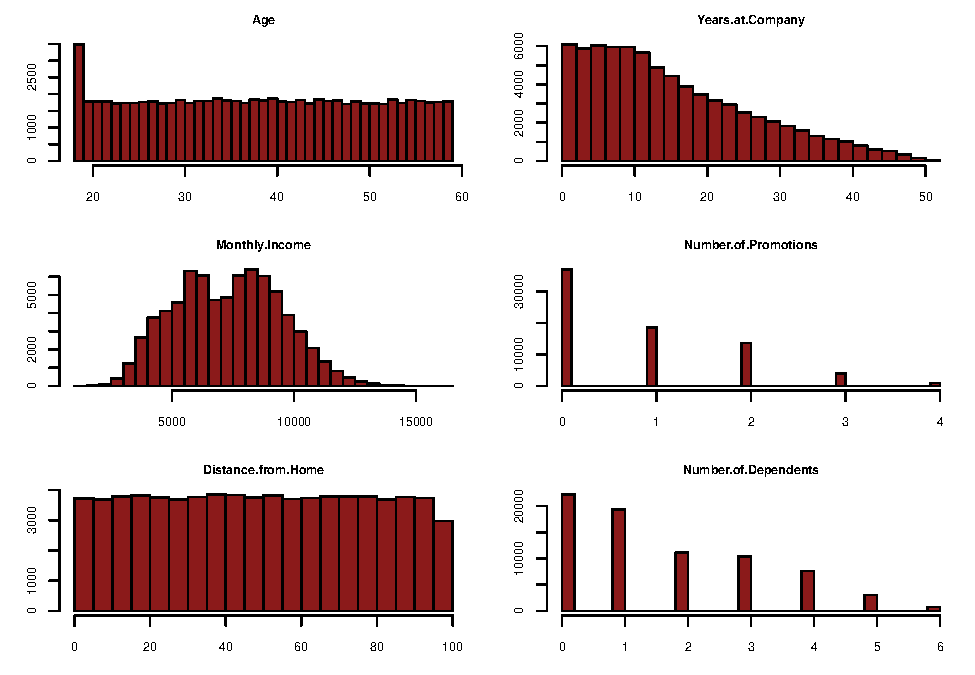
\includegraphics[width=0.65\linewidth]{figs/data_numdist-1}

\small

\begin{enumerate}
\def\labelenumi{\arabic{enumi}.}
\setcounter{enumi}{5}
\tightlist
\item
  Target Value Distribution
\end{enumerate}

The pie chart depicting attrition distribution shows that 47.5\% of
employees left the company, while 52.5\% stayed. This indicates a
relatively balanced split between those who left and those who remained.
Such a near-equal distribution suggests that significant turnover,
highlighting the need for strategies to improve retention. Understanding
the factors contributing to attrition could help in developing targeted
initiatives to retain employees and enhance overall workforce stability.

\small

\begin{Shaded}
\begin{Highlighting}[]
\CommentTok{\# Target value distribution}
\FunctionTok{par}\NormalTok{(}\AttributeTok{mfrow =} \FunctionTok{c}\NormalTok{(}\DecValTok{1}\NormalTok{, }\DecValTok{2}\NormalTok{))}
\FunctionTok{barplot}\NormalTok{(}\FunctionTok{table}\NormalTok{(data}\SpecialCharTok{$}\NormalTok{Attrition), }\AttributeTok{main =} \StringTok{"Attrition Count"}\NormalTok{, }\AttributeTok{xlab =} \StringTok{"Attrition"}\NormalTok{,}
    \AttributeTok{ylab =} \StringTok{"Count"}\NormalTok{, }\AttributeTok{col =} \FunctionTok{c}\NormalTok{(}\StringTok{"firebrick4"}\NormalTok{, }\StringTok{"rosybrown2"}\NormalTok{))}

\CommentTok{\# Target values distribution with pie chart}
\NormalTok{attrition\_table }\OtherTok{\textless{}{-}} \FunctionTok{table}\NormalTok{(data}\SpecialCharTok{$}\NormalTok{Attrition)}
\NormalTok{attrition\_df }\OtherTok{\textless{}{-}} \FunctionTok{as.data.frame}\NormalTok{(attrition\_table)}
\FunctionTok{colnames}\NormalTok{(attrition\_df) }\OtherTok{\textless{}{-}} \FunctionTok{c}\NormalTok{(}\StringTok{"Attrition"}\NormalTok{, }\StringTok{"Count"}\NormalTok{)}
\NormalTok{attrition\_df}\SpecialCharTok{$}\NormalTok{Percentage }\OtherTok{\textless{}{-}} \FunctionTok{round}\NormalTok{(}\DecValTok{100} \SpecialCharTok{*}\NormalTok{ attrition\_df}\SpecialCharTok{$}\NormalTok{Count}\SpecialCharTok{/}\FunctionTok{sum}\NormalTok{(attrition\_df}\SpecialCharTok{$}\NormalTok{Count),}
    \DecValTok{1}\NormalTok{)}
\FunctionTok{pie}\NormalTok{(attrition\_df}\SpecialCharTok{$}\NormalTok{Count, }\AttributeTok{labels =} \FunctionTok{paste}\NormalTok{(attrition\_df}\SpecialCharTok{$}\NormalTok{Attrition, }\StringTok{" {-} "}\NormalTok{, attrition\_df}\SpecialCharTok{$}\NormalTok{Percentage,}
    \StringTok{"\%"}\NormalTok{), }\AttributeTok{col =} \FunctionTok{c}\NormalTok{(}\StringTok{"firebrick4"}\NormalTok{, }\StringTok{"rosybrown2"}\NormalTok{), }\AttributeTok{main =} \StringTok{"Attrition Distribution"}\NormalTok{,}
    \AttributeTok{cex =} \DecValTok{1}\NormalTok{, }\AttributeTok{radius =} \DecValTok{1}\NormalTok{)}
\end{Highlighting}
\end{Shaded}

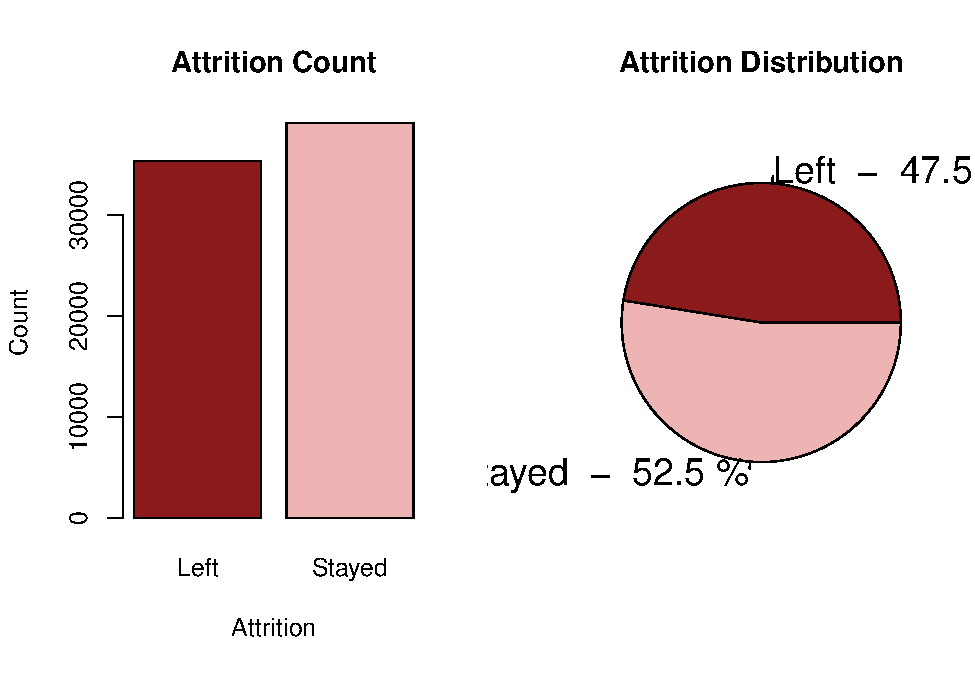
\includegraphics[width=0.65\linewidth]{figs/data_targetdist-1}

\small

\begin{enumerate}
\def\labelenumi{\arabic{enumi}.}
\setcounter{enumi}{6}
\tightlist
\item
  Outlier Analysis
\end{enumerate}

The second boxplots show the relationship between attrition and various
numerical variables: There are more outliers for longer tenures among
employees who stayed, suggesting that employees who remain with the
company for extended periods are less likely to leave. Monthly income
distributions are almost equal for both groups, but there are more
high-income outliers among those who left.This suggests that while
average income may not differ much between those who left and stayed,
higher earners are more likely to leave. Attrition appears to be more
closely linked with tenure at the company and, to some extent, with the
distribution of high-income outliers. Shorter tenures are associated
with higher attrition rates, and while income levels are generally
similar for those who leave and stay, the presence of high-income
outliers among those who leave suggests that other factors, such as job
satisfaction or career development opportunities, might be influencing
their decision to leave.

\small

\begin{Shaded}
\begin{Highlighting}[]
\CommentTok{\# Boxplot of outliers}
\FunctionTok{par}\NormalTok{(}\AttributeTok{mfrow =} \FunctionTok{c}\NormalTok{(}\DecValTok{2}\NormalTok{, }\DecValTok{3}\NormalTok{))}
\ControlFlowTok{for}\NormalTok{ (num\_var }\ControlFlowTok{in}\NormalTok{ numeric\_var\_names) \{}
    \FunctionTok{boxplot}\NormalTok{(data[[num\_var]], }\AttributeTok{main =} \FunctionTok{paste}\NormalTok{(num\_var), }\AttributeTok{xlab =} \StringTok{""}\NormalTok{, }\AttributeTok{col =} \StringTok{"firebrick4"}\NormalTok{,}
        \AttributeTok{horizontal =} \ConstantTok{TRUE}\NormalTok{)}
\NormalTok{\}}
\end{Highlighting}
\end{Shaded}

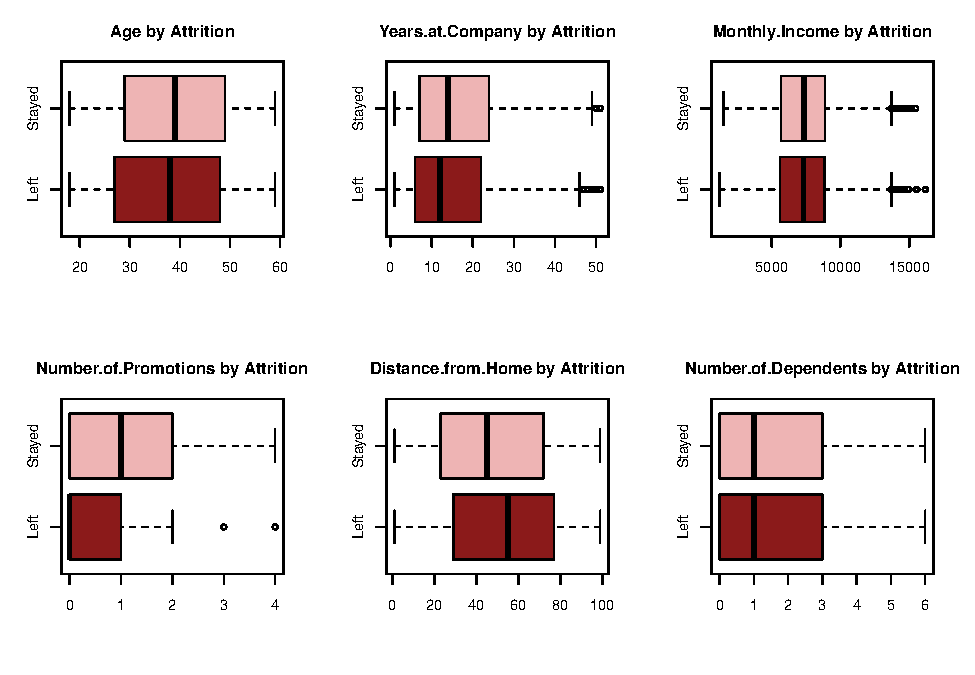
\includegraphics[width=0.75\linewidth]{figs/data_outlier-1}

\begin{Shaded}
\begin{Highlighting}[]
\CommentTok{\# Boxplots of numeric variables by Attrition}
\NormalTok{cat\_var }\OtherTok{\textless{}{-}} \StringTok{"Attrition"}
\FunctionTok{par}\NormalTok{(}\AttributeTok{mfrow =} \FunctionTok{c}\NormalTok{(}\DecValTok{2}\NormalTok{, }\DecValTok{3}\NormalTok{), }\AttributeTok{mar =} \FunctionTok{c}\NormalTok{(}\DecValTok{5}\NormalTok{, }\DecValTok{3}\NormalTok{, }\DecValTok{3}\NormalTok{, }\DecValTok{2}\NormalTok{) }\SpecialCharTok{+} \FloatTok{0.1}\NormalTok{, }\AttributeTok{cex.main =} \DecValTok{1}\NormalTok{, }\AttributeTok{cex.lab =} \FloatTok{0.9}\NormalTok{,}
    \AttributeTok{cex.axis =} \FloatTok{0.9}\NormalTok{)}
\ControlFlowTok{for}\NormalTok{ (num\_var }\ControlFlowTok{in}\NormalTok{ numeric\_var\_names) \{}
    \FunctionTok{boxplot}\NormalTok{(data[[num\_var]] }\SpecialCharTok{\textasciitilde{}}\NormalTok{ data[[cat\_var]], }\AttributeTok{main =} \FunctionTok{paste}\NormalTok{(num\_var, }\StringTok{"by Attrition"}\NormalTok{),}
        \AttributeTok{xlab =} \StringTok{""}\NormalTok{, }\AttributeTok{ylab =} \StringTok{""}\NormalTok{, }\AttributeTok{col =} \FunctionTok{c}\NormalTok{(}\StringTok{"firebrick4"}\NormalTok{, }\StringTok{"rosybrown2"}\NormalTok{), }\AttributeTok{horizontal =} \ConstantTok{TRUE}\NormalTok{,}
        \AttributeTok{names =} \FunctionTok{c}\NormalTok{(}\StringTok{"Left"}\NormalTok{, }\StringTok{"Stayed"}\NormalTok{))}
\NormalTok{\}}
\end{Highlighting}
\end{Shaded}

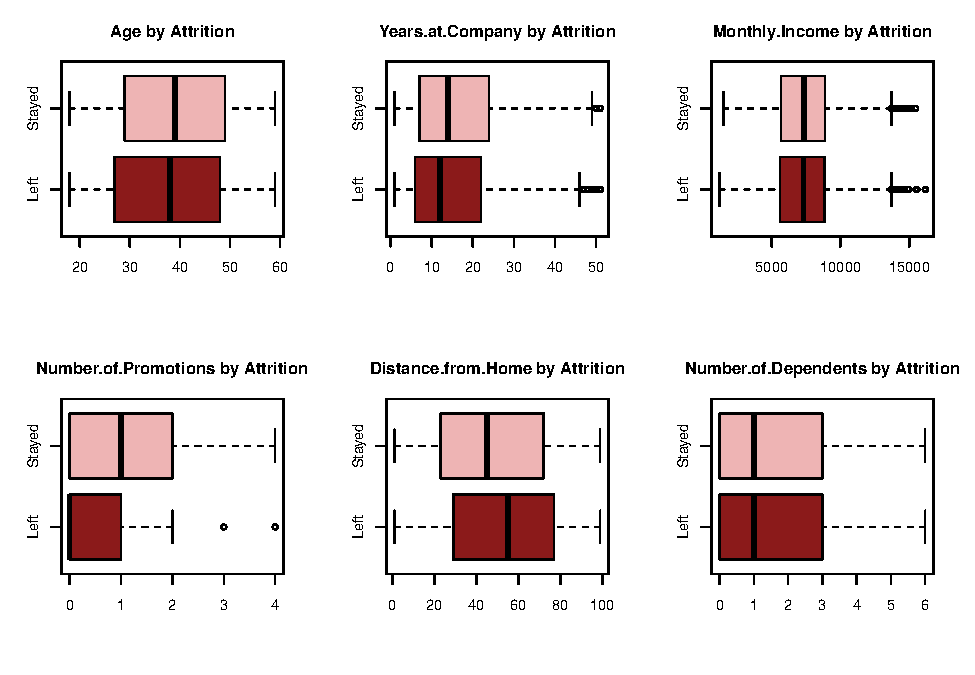
\includegraphics[width=0.75\linewidth]{figs/data_outlier-2}

\small

\small

\begin{Shaded}
\begin{Highlighting}[]
\CommentTok{\# Function to count outliers using IQR}
\NormalTok{count\_outliers }\OtherTok{\textless{}{-}} \ControlFlowTok{function}\NormalTok{(x) \{}
\NormalTok{    Q1 }\OtherTok{\textless{}{-}} \FunctionTok{quantile}\NormalTok{(x, }\FloatTok{0.25}\NormalTok{, }\AttributeTok{na.rm =} \ConstantTok{TRUE}\NormalTok{)}
\NormalTok{    Q3 }\OtherTok{\textless{}{-}} \FunctionTok{quantile}\NormalTok{(x, }\FloatTok{0.75}\NormalTok{, }\AttributeTok{na.rm =} \ConstantTok{TRUE}\NormalTok{)}
\NormalTok{    IQR }\OtherTok{\textless{}{-}}\NormalTok{ Q3 }\SpecialCharTok{{-}}\NormalTok{ Q1}
\NormalTok{    outliers }\OtherTok{\textless{}{-}}\NormalTok{ x[x }\SpecialCharTok{\textless{}}\NormalTok{ (Q1 }\SpecialCharTok{{-}} \FloatTok{1.5} \SpecialCharTok{*}\NormalTok{ IQR) }\SpecialCharTok{|}\NormalTok{ x }\SpecialCharTok{\textgreater{}}\NormalTok{ (Q3 }\SpecialCharTok{+} \FloatTok{1.5} \SpecialCharTok{*}\NormalTok{ IQR)]}
    \FunctionTok{return}\NormalTok{(}\FunctionTok{length}\NormalTok{(outliers))}
\NormalTok{\}}
\CommentTok{\# Identify and count outliers for each numeric variable}
\NormalTok{outlier\_counts }\OtherTok{\textless{}{-}} \FunctionTok{list}\NormalTok{()}
\ControlFlowTok{for}\NormalTok{ (var }\ControlFlowTok{in}\NormalTok{ numeric\_var\_names) \{}
\NormalTok{    outlier\_count }\OtherTok{\textless{}{-}} \FunctionTok{count\_outliers}\NormalTok{(data[[var]])}
\NormalTok{    outlier\_counts[[var]] }\OtherTok{\textless{}{-}}\NormalTok{ outlier\_count}
    \FunctionTok{cat}\NormalTok{(}\StringTok{"}\SpecialCharTok{\textbackslash{}n}\StringTok{Number of outliers in"}\NormalTok{, var, }\StringTok{":"}\NormalTok{, outlier\_count, }\StringTok{"}\SpecialCharTok{\textbackslash{}n}\StringTok{"}\NormalTok{)}
\NormalTok{\}}
\end{Highlighting}
\end{Shaded}

\begin{verbatim}

Number of outliers in Age : 0 

Number of outliers in Years.at.Company : 338 

Number of outliers in Monthly.Income : 65 

Number of outliers in Number.of.Promotions : 0 

Number of outliers in Distance.from.Home : 0 

Number of outliers in Number.of.Dependents : 0 
\end{verbatim}

\begin{Shaded}
\begin{Highlighting}[]
\CommentTok{\# Function to identify outliers using IQR}
\NormalTok{identify\_outliers }\OtherTok{\textless{}{-}} \ControlFlowTok{function}\NormalTok{(x) \{}
\NormalTok{    Q1 }\OtherTok{\textless{}{-}} \FunctionTok{quantile}\NormalTok{(x, }\FloatTok{0.25}\NormalTok{, }\AttributeTok{na.rm =} \ConstantTok{TRUE}\NormalTok{)}
\NormalTok{    Q3 }\OtherTok{\textless{}{-}} \FunctionTok{quantile}\NormalTok{(x, }\FloatTok{0.75}\NormalTok{, }\AttributeTok{na.rm =} \ConstantTok{TRUE}\NormalTok{)}
\NormalTok{    IQR }\OtherTok{\textless{}{-}}\NormalTok{ Q3 }\SpecialCharTok{{-}}\NormalTok{ Q1}
\NormalTok{    outliers }\OtherTok{\textless{}{-}} \FunctionTok{which}\NormalTok{(x }\SpecialCharTok{\textless{}}\NormalTok{ (Q1 }\SpecialCharTok{{-}} \FloatTok{1.5} \SpecialCharTok{*}\NormalTok{ IQR) }\SpecialCharTok{|}\NormalTok{ x }\SpecialCharTok{\textgreater{}}\NormalTok{ (Q3 }\SpecialCharTok{+} \FloatTok{1.5} \SpecialCharTok{*}\NormalTok{ IQR))  }\CommentTok{\# Return indices}
    \FunctionTok{return}\NormalTok{(outliers)}
\NormalTok{\}}
\end{Highlighting}
\end{Shaded}

\small

In methodology we used to identify and remove outlier employs the
Interquartile Range (IQR).The IQR method was used because it is simple
and effective. It focuses on the central 50\% of the data, making it
less sensitive to extreme values. It works by calculating the range
between the first quartile (Q1) and third quartile (Q3) and identifying
outliers as values falling below Q1 - 1.5 * IQR or above Q3 + 1.5 * IQR.

Functions are used to count outliers and identify their indices for each
numeric variable, subsequently removing rows with outliers to create a
non-outlier dataset. Despite this rigorous process, removing outliers
did not enhance the model's performance and instead decreased its
accuracy. This indicates that the outliers contain valuable information
crucial for the model's predictive power. Consequently, it was decided
to retain the outliers in the dataset, preserving model accuracy and
ensuring effective predictive performance.

\small

\begin{Shaded}
\begin{Highlighting}[]
\CommentTok{\# Identify and show outliers for each numeric variable and combine them}
\CommentTok{\# into single vector}
\NormalTok{outliers\_list }\OtherTok{\textless{}{-}} \FunctionTok{list}\NormalTok{()}
\NormalTok{all\_outlier\_indices }\OtherTok{\textless{}{-}} \FunctionTok{c}\NormalTok{()}
\ControlFlowTok{for}\NormalTok{ (var }\ControlFlowTok{in}\NormalTok{ numeric\_var\_names) \{}
\NormalTok{    outliers }\OtherTok{\textless{}{-}} \FunctionTok{identify\_outliers}\NormalTok{(data[[var]])}
\NormalTok{    outliers\_list[[var]] }\OtherTok{\textless{}{-}}\NormalTok{ outliers}
\NormalTok{    all\_outlier\_indices }\OtherTok{\textless{}{-}} \FunctionTok{c}\NormalTok{(all\_outlier\_indices, outliers)}
    \FunctionTok{cat}\NormalTok{(}\StringTok{"}\SpecialCharTok{\textbackslash{}n}\StringTok{Outliers in"}\NormalTok{, var, }\StringTok{":}\SpecialCharTok{\textbackslash{}n}\StringTok{"}\NormalTok{)}
    \FunctionTok{print}\NormalTok{(outliers)}
\NormalTok{\}}

\NormalTok{all\_outlier\_indices }\OtherTok{\textless{}{-}} \FunctionTok{unique}\NormalTok{(all\_outlier\_indices)}
\end{Highlighting}
\end{Shaded}

\small

\small

\begin{Shaded}
\begin{Highlighting}[]
\CommentTok{\# Remove rows with outliers}
\NormalTok{data\_nonoutlier }\OtherTok{\textless{}{-}}\NormalTok{ data[}\SpecialCharTok{{-}}\NormalTok{all\_outlier\_indices, ]}
\CommentTok{\# Print the number of rows removed and the resulting data}
\FunctionTok{cat}\NormalTok{(}\StringTok{"}\SpecialCharTok{\textbackslash{}n}\StringTok{Total number of rows removed:"}\NormalTok{, }\FunctionTok{length}\NormalTok{(all\_outlier\_indices), }\StringTok{"}\SpecialCharTok{\textbackslash{}n}\StringTok{"}\NormalTok{)}
\end{Highlighting}
\end{Shaded}

\begin{verbatim}

Total number of rows removed: 403 
\end{verbatim}

\begin{Shaded}
\begin{Highlighting}[]
\FunctionTok{cat}\NormalTok{(}\StringTok{"Original dataset rows:"}\NormalTok{, }\FunctionTok{nrow}\NormalTok{(data), }\StringTok{"}\SpecialCharTok{\textbackslash{}n}\StringTok{"}\NormalTok{)}
\end{Highlighting}
\end{Shaded}

\begin{verbatim}
Original dataset rows: 74498 
\end{verbatim}

\begin{Shaded}
\begin{Highlighting}[]
\FunctionTok{cat}\NormalTok{(}\StringTok{"Non{-}outlier dataset rows:"}\NormalTok{, }\FunctionTok{nrow}\NormalTok{(data\_nonoutlier), }\StringTok{"}\SpecialCharTok{\textbackslash{}n}\StringTok{"}\NormalTok{)}
\end{Highlighting}
\end{Shaded}

\begin{verbatim}
Non-outlier dataset rows: 74095 
\end{verbatim}

\small

\begin{enumerate}
\def\labelenumi{\arabic{enumi}.}
\setcounter{enumi}{7}
\tightlist
\item
  Transforming Numerical Variables into Categorical Variables
\end{enumerate}

This methodology effectively transforms continuous numeric variables
into categorical bins, facilitating better visualization and comparative
analysis of attrition. The use of bar charts to compare the
distributions of these categories between employees who left and those
who stayed provides clear insights into how different factors may
influence employee turnover.

Employees who do not work overtime tend to stay more than those who
leave, indicating that excessive work hours may contribute to higher
attrition rates. Married employees are less likely to leave compared to
single employees, suggesting that marital status influences retention.
Remote work and higher job levels are associated with lower attrition,
emphasizing the value of flexibility and career growth opportunities. A
good company reputation and recognition also correlate with lower
attrition, highlighting the importance of a positive work environment
and employee appreciation. The distribution across education levels,
number of dependents, and distance from home shows similar patterns for
both those who left and stayed, suggesting these factors have a moderate
impact on turnover. Understanding these patterns helps in developing
targeted strategies to improve employee satisfaction and reduce turnover
rates.

\small

\begin{Shaded}
\begin{Highlighting}[]
\CommentTok{\# Define bins for numerical variables}
\NormalTok{data\_detailed}\SpecialCharTok{$}\NormalTok{Age\_Cat }\OtherTok{\textless{}{-}} \FunctionTok{cut}\NormalTok{(data\_detailed}\SpecialCharTok{$}\NormalTok{Age, }\AttributeTok{breaks =} \FunctionTok{c}\NormalTok{(}\DecValTok{18}\NormalTok{, }\DecValTok{25}\NormalTok{, }\DecValTok{35}\NormalTok{, }\DecValTok{45}\NormalTok{,}
    \DecValTok{55}\NormalTok{, }\DecValTok{60}\NormalTok{), }\AttributeTok{labels =} \FunctionTok{c}\NormalTok{(}\StringTok{"18{-}25"}\NormalTok{, }\StringTok{"25{-}35"}\NormalTok{, }\StringTok{"35{-}45"}\NormalTok{, }\StringTok{"45{-}55"}\NormalTok{, }\StringTok{"55{-}60"}\NormalTok{), }\AttributeTok{right =} \ConstantTok{FALSE}\NormalTok{)}
\NormalTok{data\_detailed}\SpecialCharTok{$}\NormalTok{MonthlyIncome\_Cat }\OtherTok{\textless{}{-}} \FunctionTok{cut}\NormalTok{(data\_detailed}\SpecialCharTok{$}\NormalTok{Monthly.Income, }\AttributeTok{breaks =} \FunctionTok{c}\NormalTok{(}\DecValTok{0}\NormalTok{,}
    \DecValTok{3000}\NormalTok{, }\DecValTok{6000}\NormalTok{, }\DecValTok{9000}\NormalTok{, }\DecValTok{12000}\NormalTok{, }\DecValTok{15000}\NormalTok{, }\DecValTok{18000}\NormalTok{), }\AttributeTok{labels =} \FunctionTok{c}\NormalTok{(}\StringTok{"0{-}3000"}\NormalTok{, }\StringTok{"3000{-}6000"}\NormalTok{,}
    \StringTok{"6000{-}9000"}\NormalTok{, }\StringTok{"9000{-}12000"}\NormalTok{, }\StringTok{"12000{-}15000"}\NormalTok{, }\StringTok{"15000+"}\NormalTok{), }\AttributeTok{right =} \ConstantTok{FALSE}\NormalTok{)}
\NormalTok{data\_detailed}\SpecialCharTok{$}\NormalTok{DistanceFromHome\_Cat }\OtherTok{\textless{}{-}} \FunctionTok{cut}\NormalTok{(data\_detailed}\SpecialCharTok{$}\NormalTok{Distance.from.Home,}
    \AttributeTok{breaks =} \FunctionTok{c}\NormalTok{(}\DecValTok{0}\NormalTok{, }\DecValTok{20}\NormalTok{, }\DecValTok{40}\NormalTok{, }\DecValTok{60}\NormalTok{, }\DecValTok{80}\NormalTok{, }\DecValTok{100}\NormalTok{), }\AttributeTok{labels =} \FunctionTok{c}\NormalTok{(}\StringTok{"0{-}20"}\NormalTok{, }\StringTok{"20{-}40"}\NormalTok{, }\StringTok{"40{-}60"}\NormalTok{,}
        \StringTok{"60{-}80"}\NormalTok{, }\StringTok{"80{-}100"}\NormalTok{), }\AttributeTok{right =} \ConstantTok{FALSE}\NormalTok{)}
\NormalTok{data\_detailed}\SpecialCharTok{$}\NormalTok{YearsAtCompany\_Cat }\OtherTok{\textless{}{-}} \FunctionTok{cut}\NormalTok{(data\_detailed}\SpecialCharTok{$}\NormalTok{Years.at.Company, }\AttributeTok{breaks =} \FunctionTok{c}\NormalTok{(}\DecValTok{0}\NormalTok{,}
    \DecValTok{10}\NormalTok{, }\DecValTok{20}\NormalTok{, }\DecValTok{30}\NormalTok{, }\DecValTok{40}\NormalTok{, }\DecValTok{50}\NormalTok{, }\DecValTok{60}\NormalTok{), }\AttributeTok{labels =} \FunctionTok{c}\NormalTok{(}\StringTok{"0{-}10"}\NormalTok{, }\StringTok{"10{-}20"}\NormalTok{, }\StringTok{"20{-}30"}\NormalTok{, }\StringTok{"30{-}40"}\NormalTok{,}
    \StringTok{"40{-}50"}\NormalTok{, }\StringTok{"50{-}60"}\NormalTok{), }\AttributeTok{right =} \ConstantTok{FALSE}\NormalTok{)}

\CommentTok{\# Exclude numerical columns}
\NormalTok{exclude\_columns }\OtherTok{\textless{}{-}} \FunctionTok{c}\NormalTok{(}\StringTok{"Age"}\NormalTok{, }\StringTok{"Monthly.Income"}\NormalTok{, }\StringTok{"Distance.from.Home"}\NormalTok{, }\StringTok{"Years.at.Company"}\NormalTok{,}
    \StringTok{"Attrition"}\NormalTok{)}
\NormalTok{exclude\_columns1 }\OtherTok{\textless{}{-}} \FunctionTok{c}\NormalTok{(}\StringTok{"Age"}\NormalTok{, }\StringTok{"Monthly.Income"}\NormalTok{, }\StringTok{"Distance.from.Home"}\NormalTok{, }\StringTok{"Years.at.Company"}\NormalTok{)}
\CommentTok{\# Create data for correlation matrix}
\NormalTok{data\_corr }\OtherTok{\textless{}{-}}\NormalTok{ data\_detailed[, }\SpecialCharTok{!}\FunctionTok{names}\NormalTok{(data\_detailed) }\SpecialCharTok{\%in\%}\NormalTok{ exclude\_columns1]}
\NormalTok{data\_corr }\OtherTok{\textless{}{-}}\NormalTok{ data\_corr[, }\FunctionTok{c}\NormalTok{(}\FunctionTok{setdiff}\NormalTok{(}\FunctionTok{names}\NormalTok{(data\_corr), }\StringTok{"Attrition"}\NormalTok{), }\StringTok{"Attrition"}\NormalTok{)]}

\CommentTok{\# Plotting with target feature after transform numerical variables into}
\CommentTok{\# categorical}
\FunctionTok{par}\NormalTok{(}\AttributeTok{mfrow =} \FunctionTok{c}\NormalTok{(}\DecValTok{3}\NormalTok{, }\DecValTok{4}\NormalTok{), }\AttributeTok{mar =} \FunctionTok{c}\NormalTok{(}\DecValTok{3}\NormalTok{, }\DecValTok{3}\NormalTok{, }\DecValTok{2}\NormalTok{, }\DecValTok{2}\NormalTok{) }\SpecialCharTok{+} \FloatTok{0.1}\NormalTok{)}
\ControlFlowTok{for}\NormalTok{ (col }\ControlFlowTok{in} \FunctionTok{setdiff}\NormalTok{(}\FunctionTok{names}\NormalTok{(data\_detailed), exclude\_columns)) \{}
\NormalTok{    table\_left }\OtherTok{\textless{}{-}} \FunctionTok{table}\NormalTok{(data\_detailed[data\_detailed}\SpecialCharTok{$}\NormalTok{Attrition }\SpecialCharTok{==} \StringTok{"Left"}\NormalTok{,}
\NormalTok{        col])}
\NormalTok{    table\_stayed }\OtherTok{\textless{}{-}} \FunctionTok{table}\NormalTok{(data\_detailed[data\_detailed}\SpecialCharTok{$}\NormalTok{Attrition }\SpecialCharTok{==} \StringTok{"Stayed"}\NormalTok{,}
\NormalTok{        col])}
    \FunctionTok{barplot}\NormalTok{(}\FunctionTok{rbind}\NormalTok{(table\_left, table\_stayed), }\AttributeTok{beside =} \ConstantTok{TRUE}\NormalTok{, }\AttributeTok{main =} \FunctionTok{paste}\NormalTok{(col),}
        \AttributeTok{xlab =} \StringTok{""}\NormalTok{, }\AttributeTok{col =} \FunctionTok{c}\NormalTok{(}\StringTok{"firebrick4"}\NormalTok{, }\StringTok{"rosybrown2"}\NormalTok{), }\AttributeTok{cex.names =} \FloatTok{0.9}\NormalTok{,}
        \AttributeTok{cex.main =} \FloatTok{0.9}\NormalTok{, }\AttributeTok{cex.axis =} \FloatTok{0.9}\NormalTok{)}
\NormalTok{\}}
\end{Highlighting}
\end{Shaded}

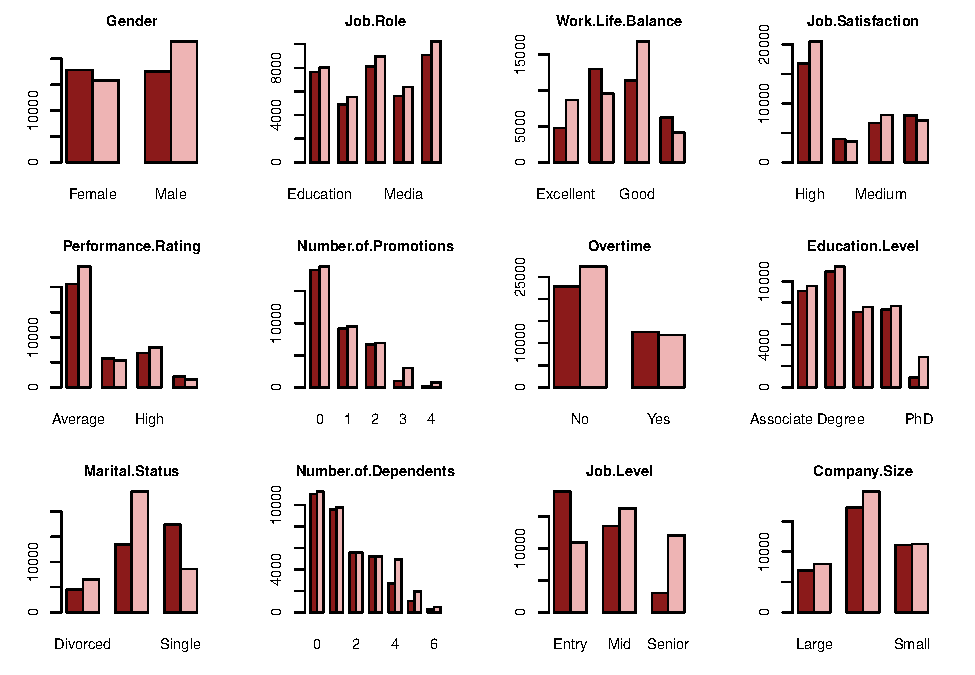
\includegraphics[width=0.75\linewidth]{figs/data_transform-1}
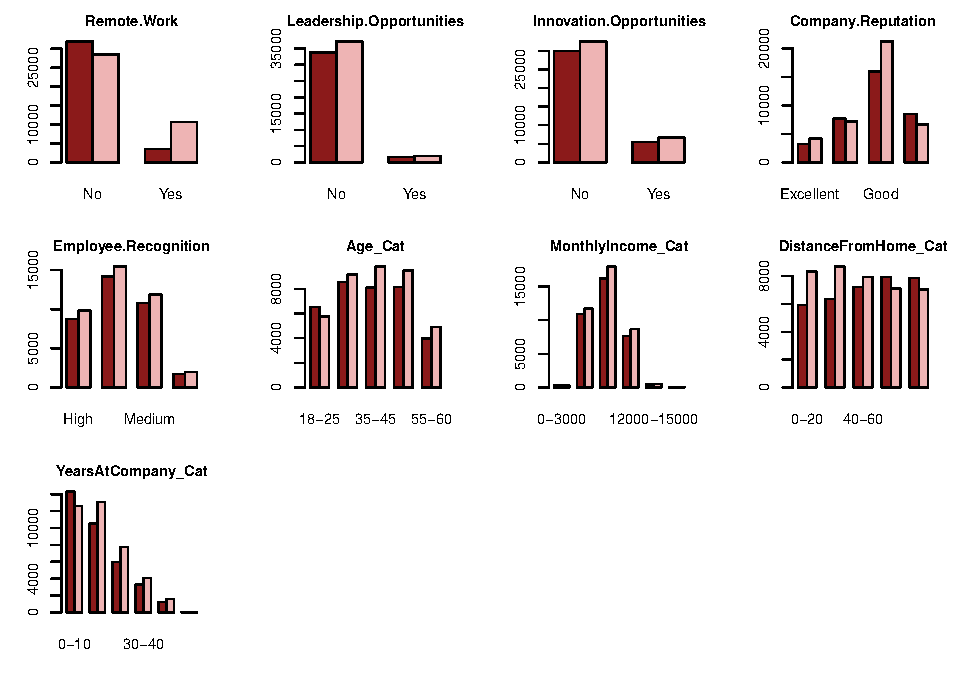
\includegraphics[width=0.75\linewidth]{figs/data_transform-2}

\small

\begin{enumerate}
\def\labelenumi{\arabic{enumi}.}
\setcounter{enumi}{8}
\tightlist
\item
  Checking Correlation
\end{enumerate}

In order to look at the correlation between variables and their effect
on Attrition, ordinal and label encoding are used on categorical
variables, followed by generating a correlation matrix and visualizing
it.

Ordinal mapping converts variables with inherent order, such as
Work-Life Balance and Job Satisfaction, into numeric values to preserve
their ordinal nature, enabling meaningful numerical analysis. Label
encoding is applied to unordered categorical variables, converting them
into numeric values necessary for numerical analyses.

Additionally, numeric variables were converted to categorical bins
previous code and then encoded to avoid issues related to large or small
numeric values and to standardize the data format, ensuring consistency
in the correlation analysis. By encoding the data, we aim to avoid
disproportionate influence from large or small values and ensure each
variable contributes equally to the analysis. The correlation matrix
calculates pairwise correlation coefficients, helping to understand the
linear relationships between variables. The correlation plot visually
represents these relationships, using colors and numbers to indicate the
strength and direction of correlations.So this process prepares the
dataset for sophisticated analysis, aids in feature selection,
identifies multicollinearity issues, and providing insights into complex
variable relationships.

However, it is important to note that this method may not capture the
full complexity of relationships that exist in the original numeric
data.

\small

\begin{Shaded}
\begin{Highlighting}[]
\CommentTok{\# Ordinal mappings}
\NormalTok{balance.map }\OtherTok{\textless{}{-}} \FunctionTok{c}\NormalTok{(}\AttributeTok{Poor =} \DecValTok{1}\NormalTok{, }\AttributeTok{Fair =} \DecValTok{2}\NormalTok{, }\AttributeTok{Good =} \DecValTok{3}\NormalTok{, }\AttributeTok{Excellent =} \DecValTok{4}\NormalTok{)}
\NormalTok{data\_corr}\SpecialCharTok{$}\NormalTok{Work.Life.Balance }\OtherTok{\textless{}{-}}\NormalTok{ balance.map[}\FunctionTok{as.character}\NormalTok{(data\_corr}\SpecialCharTok{$}\NormalTok{Work.Life.Balance)]}

\NormalTok{satisfaction.map }\OtherTok{\textless{}{-}} \FunctionTok{c}\NormalTok{(}\AttributeTok{Low =} \DecValTok{1}\NormalTok{, }\AttributeTok{Medium =} \DecValTok{2}\NormalTok{, }\AttributeTok{High =} \DecValTok{3}\NormalTok{, }\StringTok{\textasciigrave{}}\AttributeTok{Very High}\StringTok{\textasciigrave{}} \OtherTok{=} \DecValTok{4}\NormalTok{)}
\NormalTok{data\_corr}\SpecialCharTok{$}\NormalTok{Job.Satisfaction }\OtherTok{\textless{}{-}}\NormalTok{ satisfaction.map[}\FunctionTok{as.character}\NormalTok{(data\_corr}\SpecialCharTok{$}\NormalTok{Job.Satisfaction)]}

\NormalTok{performance.map }\OtherTok{\textless{}{-}} \FunctionTok{c}\NormalTok{(}\AttributeTok{Low =} \DecValTok{1}\NormalTok{, }\StringTok{\textasciigrave{}}\AttributeTok{Below Average}\StringTok{\textasciigrave{}} \OtherTok{=} \DecValTok{2}\NormalTok{, }\AttributeTok{Average =} \DecValTok{3}\NormalTok{, }\AttributeTok{High =} \DecValTok{4}\NormalTok{)}
\NormalTok{data\_corr}\SpecialCharTok{$}\NormalTok{Performance.Rating }\OtherTok{\textless{}{-}}\NormalTok{ performance.map[}\FunctionTok{as.character}\NormalTok{(data\_corr}\SpecialCharTok{$}\NormalTok{Performance.Rating)]}

\NormalTok{level.map }\OtherTok{\textless{}{-}} \FunctionTok{c}\NormalTok{(}\AttributeTok{Entry =} \DecValTok{1}\NormalTok{, }\AttributeTok{Mid =} \DecValTok{2}\NormalTok{, }\AttributeTok{Senior =} \DecValTok{3}\NormalTok{)}
\NormalTok{data\_corr}\SpecialCharTok{$}\NormalTok{Job.Level }\OtherTok{\textless{}{-}}\NormalTok{ level.map[}\FunctionTok{as.character}\NormalTok{(data\_corr}\SpecialCharTok{$}\NormalTok{Job.Level)]}

\NormalTok{reputation.map }\OtherTok{\textless{}{-}} \FunctionTok{c}\NormalTok{(}\AttributeTok{Poor =} \DecValTok{1}\NormalTok{, }\AttributeTok{Fair =} \DecValTok{2}\NormalTok{, }\AttributeTok{Good =} \DecValTok{3}\NormalTok{, }\AttributeTok{Excellent =} \DecValTok{4}\NormalTok{)}
\NormalTok{data\_corr}\SpecialCharTok{$}\NormalTok{Company.Reputation }\OtherTok{\textless{}{-}}\NormalTok{ reputation.map[}\FunctionTok{as.character}\NormalTok{(data\_corr}\SpecialCharTok{$}\NormalTok{Company.Reputation)]}

\NormalTok{recognition.map }\OtherTok{\textless{}{-}} \FunctionTok{c}\NormalTok{(}\AttributeTok{Low =} \DecValTok{1}\NormalTok{, }\AttributeTok{Medium =} \DecValTok{2}\NormalTok{, }\AttributeTok{High =} \DecValTok{3}\NormalTok{, }\StringTok{\textasciigrave{}}\AttributeTok{Very High}\StringTok{\textasciigrave{}} \OtherTok{=} \DecValTok{4}\NormalTok{)}
\NormalTok{data\_corr}\SpecialCharTok{$}\NormalTok{Employee.Recognition }\OtherTok{\textless{}{-}}\NormalTok{ recognition.map[}\FunctionTok{as.character}\NormalTok{(data\_corr}\SpecialCharTok{$}\NormalTok{Employee.Recognition)]}

\NormalTok{size.map }\OtherTok{\textless{}{-}} \FunctionTok{c}\NormalTok{(}\AttributeTok{Small =} \DecValTok{1}\NormalTok{, }\AttributeTok{Medium =} \DecValTok{2}\NormalTok{, }\AttributeTok{Large =} \DecValTok{3}\NormalTok{)}
\NormalTok{data\_corr}\SpecialCharTok{$}\NormalTok{Company.Size }\OtherTok{\textless{}{-}}\NormalTok{ size.map[}\FunctionTok{as.character}\NormalTok{(data\_corr}\SpecialCharTok{$}\NormalTok{Company.Size)]}

\CommentTok{\# Perform label encoding for the columns that are not mapped ordinally}
\NormalTok{categoric\_vars\_enc }\OtherTok{\textless{}{-}} \FunctionTok{sapply}\NormalTok{(data\_corr, }\ControlFlowTok{function}\NormalTok{(x) }\FunctionTok{is.factor}\NormalTok{(x) }\SpecialCharTok{||} \FunctionTok{is.character}\NormalTok{(x))}
\ControlFlowTok{for}\NormalTok{ (var }\ControlFlowTok{in} \FunctionTok{names}\NormalTok{(data\_corr)[categoric\_vars\_enc]) \{}
    \ControlFlowTok{if}\NormalTok{ (}\SpecialCharTok{!}\NormalTok{(var }\SpecialCharTok{\%in\%} \FunctionTok{c}\NormalTok{(}\StringTok{"Work.Life.Balance"}\NormalTok{, }\StringTok{"Job.Satisfaction"}\NormalTok{, }\StringTok{"Performance.Rating"}\NormalTok{,}
        \StringTok{"Job.Level"}\NormalTok{, }\StringTok{"Company.Reputation"}\NormalTok{, }\StringTok{"Employee.Recognition"}\NormalTok{, }\StringTok{"Company.Size"}\NormalTok{))) \{}
\NormalTok{        data\_corr[[var]] }\OtherTok{\textless{}{-}} \FunctionTok{as.numeric}\NormalTok{(}\FunctionTok{factor}\NormalTok{(data\_corr[[var]]))}
\NormalTok{    \}}
\NormalTok{\}}
\CommentTok{\# Define cor matrix}
\NormalTok{cor\_matrix }\OtherTok{\textless{}{-}} \FunctionTok{cor}\NormalTok{(data\_corr)}
\CommentTok{\# Correlation plot}
\FunctionTok{corrplot}\NormalTok{(cor\_matrix, }\AttributeTok{method =} \StringTok{"color"}\NormalTok{, }\AttributeTok{type =} \StringTok{"upper"}\NormalTok{, }\AttributeTok{tl.col =} \StringTok{"black"}\NormalTok{,}
    \AttributeTok{tl.srt =} \DecValTok{45}\NormalTok{, }\AttributeTok{addCoef.col =} \StringTok{"black"}\NormalTok{, }\AttributeTok{number.cex =} \FloatTok{0.5}\NormalTok{, }\AttributeTok{tl.cex =} \FloatTok{0.5}\NormalTok{)}
\end{Highlighting}
\end{Shaded}

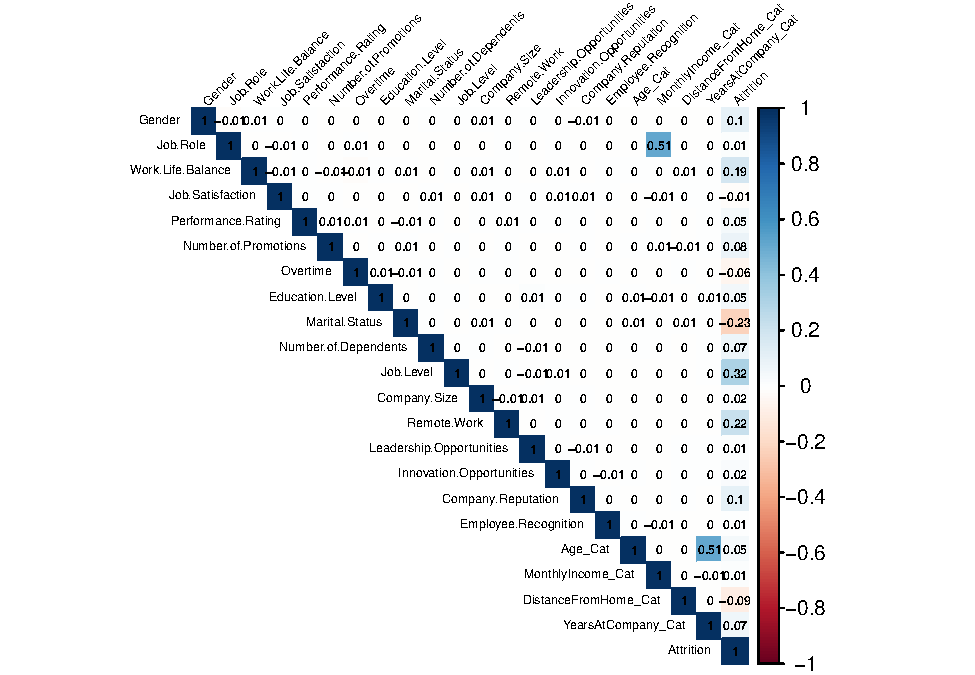
\includegraphics[width=0.8\linewidth]{figs/data_corr-1}

\small

There is positive correlation between job role and monthly income
(0.51), indicating that higher job roles (Media 4,Technology 5) are
associated with higher incomes. Work-life balance shows a positive
correlation with attrition (0.19), suggesting that employees with better
work-life balance are more likely to stay.This emphasizes the importance
of promoting a healthy work-life balance to reduce turnover rates. There
is also a notable negative correlation between marital status and
attrition (-0.23), indicating that married employees are less likely to
leave the company. Remote work has a moderate negative correlation with
attrition (-0.22), suggesting that employees who can work remotely are
more likely to stay.The flexibility offered by remote work arrangements
can be a significant factor in retaining employees, especially in the
current global context where remote work has become more prevalent. Job
level also shows a notable negative correlation with attrition (-0.32),
implying that higher job levels are associated with lower attrition
rates.This could be due to increased job satisfaction, responsibility,
and rewards that come with higher-level positions, making employees more
likely to stay. Additionally, there is a weak negative correlation
between distance from home and attrition (-0.09), and a very weak
positive correlation between years at the company and attrition (0.07).
These insights highlight which factors are more strongly related to
employee turnover, providing valuable information for developing
targeted retention strategies.

\section{Data Preparation}\label{data-preparation}

After completing the data analysis steps, it is necessary to prepare the
data for model development.

\subsection{Handling Categorical
Features}\label{handling-categorical-features}

In order to use the categorical features in the model, we need to
convert categorical features to numeric (ordinal or nominal)
representations.

\small

\begin{Shaded}
\begin{Highlighting}[]
\CommentTok{\# Ordinal mappings:}
\NormalTok{data}\SpecialCharTok{$}\NormalTok{Work.Life.Balance }\OtherTok{\textless{}{-}}\NormalTok{ balance.map[}\FunctionTok{as.numeric}\NormalTok{(data}\SpecialCharTok{$}\NormalTok{Work.Life.Balance)]}
\NormalTok{data}\SpecialCharTok{$}\NormalTok{Job.Satisfaction }\OtherTok{\textless{}{-}}\NormalTok{ satisfaction.map[}\FunctionTok{as.numeric}\NormalTok{(data}\SpecialCharTok{$}\NormalTok{Job.Satisfaction)]}
\NormalTok{data}\SpecialCharTok{$}\NormalTok{Performance.Rating }\OtherTok{\textless{}{-}}\NormalTok{ performance.map[}\FunctionTok{as.numeric}\NormalTok{(data}\SpecialCharTok{$}\NormalTok{Performance.Rating)]}
\NormalTok{data}\SpecialCharTok{$}\NormalTok{Job.Level }\OtherTok{\textless{}{-}}\NormalTok{ level.map[}\FunctionTok{as.numeric}\NormalTok{(data}\SpecialCharTok{$}\NormalTok{Job.Level)]}
\NormalTok{data}\SpecialCharTok{$}\NormalTok{Company.Reputation }\OtherTok{\textless{}{-}}\NormalTok{ reputation.map[}\FunctionTok{as.numeric}\NormalTok{(data}\SpecialCharTok{$}\NormalTok{Company.Reputation)]}
\NormalTok{data}\SpecialCharTok{$}\NormalTok{Employee.Recognition }\OtherTok{\textless{}{-}}\NormalTok{ recognition.map[}\FunctionTok{as.numeric}\NormalTok{(data}\SpecialCharTok{$}\NormalTok{Employee.Recognition)]}
\NormalTok{data}\SpecialCharTok{$}\NormalTok{Company.Size }\OtherTok{\textless{}{-}}\NormalTok{ size.map[}\FunctionTok{as.numeric}\NormalTok{(data}\SpecialCharTok{$}\NormalTok{Company.Size)]}

\CommentTok{\# Nominal mappings: Create dummy variables for nominal data}
\NormalTok{data\_numeric }\OtherTok{\textless{}{-}} \FunctionTok{model.matrix}\NormalTok{(}\SpecialCharTok{\textasciitilde{}}\NormalTok{., }\AttributeTok{data =}\NormalTok{ data)}
\CommentTok{\# Convert the resulting matrix back to a data frame}
\NormalTok{data\_numeric }\OtherTok{\textless{}{-}} \FunctionTok{as.data.frame}\NormalTok{(data\_numeric)[, }\SpecialCharTok{{-}}\DecValTok{1}\NormalTok{]  }\CommentTok{\# {-}1 to remove the intercept}
\end{Highlighting}
\end{Shaded}

\small

\subsection{Normalization}\label{normalization}

\small

\begin{Shaded}
\begin{Highlighting}[]
\NormalTok{normalize }\OtherTok{\textless{}{-}} \ControlFlowTok{function}\NormalTok{(x) \{}
    \FunctionTok{return}\NormalTok{((x }\SpecialCharTok{{-}} \FunctionTok{min}\NormalTok{(x))}\SpecialCharTok{/}\NormalTok{(}\FunctionTok{max}\NormalTok{(x) }\SpecialCharTok{{-}} \FunctionTok{min}\NormalTok{(x)))}
\NormalTok{\}}

\NormalTok{data\_normalized }\OtherTok{\textless{}{-}} \FunctionTok{as.data.frame}\NormalTok{(}\FunctionTok{lapply}\NormalTok{(data\_numeric, normalize))}
\end{Highlighting}
\end{Shaded}

\small

\subsection{Train-Test-Split}\label{train-test-split}

\small

\begin{Shaded}
\begin{Highlighting}[]
\FunctionTok{set.seed}\NormalTok{(}\DecValTok{123}\NormalTok{)}
\NormalTok{trainIndex }\OtherTok{\textless{}{-}} \FunctionTok{sample}\NormalTok{(}\DecValTok{1}\SpecialCharTok{:}\FunctionTok{nrow}\NormalTok{(data\_normalized), }\FloatTok{0.8} \SpecialCharTok{*} \FunctionTok{nrow}\NormalTok{(data\_normalized))}

\CommentTok{\# 80\% of data is used for training}
\NormalTok{train.data }\OtherTok{\textless{}{-}}\NormalTok{ data\_normalized[trainIndex, ]}

\CommentTok{\# 20\% of data is used for testing}
\NormalTok{test.data }\OtherTok{\textless{}{-}}\NormalTok{ data\_normalized[}\SpecialCharTok{{-}}\NormalTok{trainIndex, ]}
\end{Highlighting}
\end{Shaded}

\small

\small

\begin{Shaded}
\begin{Highlighting}[]
\CommentTok{\# Splitting data into features and target:}
\NormalTok{X.train }\OtherTok{\textless{}{-}}\NormalTok{ train.data[, }\SpecialCharTok{!}\NormalTok{(}\FunctionTok{colnames}\NormalTok{(data\_normalized) }\SpecialCharTok{\%in\%} \FunctionTok{c}\NormalTok{(}\StringTok{"Employee.ID"}\NormalTok{,}
    \StringTok{"AttritionStayed"}\NormalTok{))]}
\NormalTok{y.train }\OtherTok{\textless{}{-}}\NormalTok{ train.data}\SpecialCharTok{$}\NormalTok{AttritionStayed}

\NormalTok{X.test }\OtherTok{\textless{}{-}}\NormalTok{ test.data[, }\SpecialCharTok{!}\NormalTok{(}\FunctionTok{colnames}\NormalTok{(data\_normalized) }\SpecialCharTok{\%in\%} \FunctionTok{c}\NormalTok{(}\StringTok{"Employee.ID"}\NormalTok{, }\StringTok{"AttritionStayed"}\NormalTok{))]}
\NormalTok{y.test }\OtherTok{\textless{}{-}}\NormalTok{ test.data}\SpecialCharTok{$}\NormalTok{AttritionStayed}
\end{Highlighting}
\end{Shaded}

\small

Now, we can split the dataset for modelling.

Before moving to modelling step, it is beneficial to check the
dimensions and balance of the datasets.

\begin{itemize}
\item
  Number of samples in train data: 59598
\item
  Number of samples in test data: 14900
\item
  Proportion of stayed employees for train data:
\end{itemize}

\small

\begin{verbatim}
y.train
        0         1 
0.4733213 0.5266787 
\end{verbatim}

\small

\begin{itemize}
\tightlist
\item
  Proportion of stayed employees for test data:
\end{itemize}

\small

\begin{verbatim}
y.test
       0        1 
0.480604 0.519396 
\end{verbatim}

\small

We can observe that the train and test datasets are balanced within
themselves. Also the train data is representative of test data.

\section{Predictive Classification
Models}\label{predictive-classification-models}

Predictive classification models are a type of machine learning
algorithm used to predict the category or class label of new, unseen
instances based on historical data. These models are trained using a
labelled dataset where the input features (independent variables) are
associated with known class labels (dependent variable). The goal of the
model is to learn the relationship between the features and the class
labels so that it can accurately classify new data points into one of
the predefined categories.

In this project we aim to find the risk of an employee leaving the
company (class 0) and the factors affecting employee retention. So we
will develop several classification models and examine their
performances.

\subsection{Logistic Regression}\label{logistic-regression}

The logistic regression model estimates the odds of the dependent
variable occurring and applies the logit (log-odds) transformation to
express this relationship.

\subsubsection{Basic Logistic
Classifier}\label{basic-logistic-classifier}

\small

\begin{Shaded}
\begin{Highlighting}[]
\CommentTok{\# First of all we check the model statistics with all the features}
\NormalTok{glm.FULL }\OtherTok{\textless{}{-}} \FunctionTok{glm}\NormalTok{(y.train }\SpecialCharTok{\textasciitilde{}}\NormalTok{ ., }\AttributeTok{data =}\NormalTok{ X.train, }\AttributeTok{family =}\NormalTok{ binomial)}
\FunctionTok{summary}\NormalTok{(glm.FULL)}
\end{Highlighting}
\end{Shaded}

\begin{verbatim}

Call:
glm(formula = y.train ~ ., family = binomial, data = X.train)

Coefficients:
                                  Estimate Std. Error z value Pr(>|z|)    
(Intercept)                      -0.553730   0.064437  -8.593  < 2e-16 ***
Age                               0.229757   0.039315   5.844 5.10e-09 ***
GenderMale                        0.543694   0.019788  27.476  < 2e-16 ***
Years.at.Company                  0.654574   0.051922  12.607  < 2e-16 ***
Job.RoleFinance                   0.109910   0.046309   2.373 0.017625 *  
Job.RoleHealthcare                0.061875   0.040506   1.528 0.126628    
Job.RoleMedia                     0.106027   0.034483   3.075 0.002107 ** 
Job.RoleTechnology                0.098439   0.046401   2.121 0.033880 *  
Monthly.Income                    0.018438   0.117791   0.157 0.875614    
Work.Life.Balance                -0.565409   0.031321 -18.052  < 2e-16 ***
Job.Satisfaction                 -0.365624   0.024033 -15.213  < 2e-16 ***
Performance.Rating               -0.289214   0.030814  -9.386  < 2e-16 ***
Number.of.Promotions              0.928255   0.039924  23.250  < 2e-16 ***
OvertimeYes                      -0.336407   0.020902 -16.095  < 2e-16 ***
Distance.from.Home               -0.886487   0.033969 -26.097  < 2e-16 ***
Education.LevelBachelor.s.Degree -0.035818   0.026276  -1.363 0.172835    
Education.LevelHigh.School        0.001582   0.029370   0.054 0.957050    
Education.LevelMaster.s.Degree   -0.006862   0.029087  -0.236 0.813509    
Education.LevelPhD                1.506973   0.053149  28.354  < 2e-16 ***
Marital.StatusMarried             0.257001   0.028268   9.092  < 2e-16 ***
Marital.StatusSingle             -1.409863   0.030515 -46.203  < 2e-16 ***
Number.of.Dependents              0.842765   0.038204  22.060  < 2e-16 ***
Job.Level                         2.292477   0.028636  80.056  < 2e-16 ***
Company.Size                     -0.193325   0.027989  -6.907 4.94e-12 ***
Remote.WorkYes                    1.635385   0.027848  58.726  < 2e-16 ***
Leadership.OpportunitiesYes       0.162824   0.045057   3.614 0.000302 ***
Innovation.OpportunitiesYes       0.127904   0.026574   4.813 1.49e-06 ***
Company.Reputation               -0.342783   0.033757 -10.154  < 2e-16 ***
Employee.Recognition             -0.003910   0.034468  -0.113 0.909677    
---
Signif. codes:  0 '***' 0.001 '**' 0.01 '*' 0.05 '.' 0.1 ' ' 1

(Dispersion parameter for binomial family taken to be 1)

    Null deviance: 82451  on 59597  degrees of freedom
Residual deviance: 62455  on 59569  degrees of freedom
AIC: 62513

Number of Fisher Scoring iterations: 4
\end{verbatim}

\small

The above model statistics indicate that p-value of Employee Recognition
is above 0.5 indicating that this feature is insignificant to the
results. Additionally, some Job.Roles and Monthly. Income also have high
p-values indicating that their effect on Attrition is less significant
compared to other features. However, for now we would like to keep all
the features in the model and apply feature selection later.

In order to understand how well the model fits the data we can make use
of \(R^2\) statistics. \(R^2\) provides an indication of how well the
independent variables in the model explain the variability of the
dependent variable. A higher \(R^2\) value indicates a better fit of the
model to the data. The formula for \(R^2\) is:

\[ R^2 = 1 - \frac{RSS}{ESS} \]

Where:

\begin{itemize}
\tightlist
\item
  \({RSS}\) is the sum of squares of the residuals (the differences
  between observed and predicted values), i.e.~the deviance of the
  fitted model
\item
  \({ESS}\) is the total sum of squares due to regression (the
  differences between the observed values and the mean of the observed
  values)
\end{itemize}

\small

\begin{Shaded}
\begin{Highlighting}[]
\NormalTok{R2 }\OtherTok{\textless{}{-}} \DecValTok{1} \SpecialCharTok{{-}}\NormalTok{ (}\FunctionTok{summary}\NormalTok{(glm.FULL)}\SpecialCharTok{$}\NormalTok{deviance}\SpecialCharTok{/}\FunctionTok{summary}\NormalTok{(glm.FULL)}\SpecialCharTok{$}\NormalTok{null.deviance)}
\NormalTok{R2}
\end{Highlighting}
\end{Shaded}

\begin{verbatim}
[1] 0.2425186
\end{verbatim}

\small

With the full model the value of \(R^2\) 0.2425186 indicates that
approximately 24.2518642\% of the variance in the target can be
explained by the features in the model. Since 24.2518642\% is relatively
low, it suggests that the model is not capturing much of the underlying
pattern in the data.

Multicollinearity can be a reason for a low \(R^2\) value, as it can
make it difficult to determine the individual effect of each predictor
on the target. Calculating the Variance Inflation Factor (VIF) can help
to check for multicollinearity among the features.

\small

\begin{Shaded}
\begin{Highlighting}[]
\NormalTok{vif.FULL }\OtherTok{\textless{}{-}} \FunctionTok{data.frame}\NormalTok{(}\AttributeTok{features =} \FunctionTok{names}\NormalTok{(}\FunctionTok{vif}\NormalTok{(glm.FULL)), }\AttributeTok{VIF =} \FunctionTok{vif}\NormalTok{(glm.FULL),}
    \AttributeTok{row.names =} \ConstantTok{NULL}\NormalTok{)}
\NormalTok{vif.FULL[}\FunctionTok{order}\NormalTok{(}\SpecialCharTok{{-}}\NormalTok{vif.FULL}\SpecialCharTok{$}\NormalTok{VIF), ]}
\end{Highlighting}
\end{Shaded}

\begin{verbatim}
                           features      VIF
7                Job.RoleTechnology 4.317840
5                Job.RoleHealthcare 3.028354
8                    Monthly.Income 3.014476
4                   Job.RoleFinance 2.699408
20             Marital.StatusSingle 2.164088
19            Marital.StatusMarried 2.085912
6                     Job.RoleMedia 1.682568
15 Education.LevelBachelor.s.Degree 1.528098
17   Education.LevelMaster.s.Degree 1.434283
16       Education.LevelHigh.School 1.424799
3                  Years.at.Company 1.405468
1                               Age 1.403168
18               Education.LevelPhD 1.124677
22                        Job.Level 1.098028
24                   Remote.WorkYes 1.060436
2                        GenderMale 1.013155
14               Distance.from.Home 1.011754
12             Number.of.Promotions 1.009919
21             Number.of.Dependents 1.009231
9                 Work.Life.Balance 1.007059
10                 Job.Satisfaction 1.005314
13                      OvertimeYes 1.005171
27               Company.Reputation 1.002671
11               Performance.Rating 1.001850
23                     Company.Size 1.001579
25      Leadership.OpportunitiesYes 1.000932
28             Employee.Recognition 1.000568
26      Innovation.OpportunitiesYes 1.000566
\end{verbatim}

\small

A VIF value of 1 indicates no correlation, values between 1 and 5
indicate moderate correlation and values above 5 suggest significant
multicollinearity, which can lead to unreliable coefficient estimates.
Most variables have VIF values close to 1, indicating very low or no
multicollinearity. A few variables have VIF values between 1 and 5,
suggesting moderate multicollinearity, which may not pose serious issues
but should be monitored. These variables include Job.RoleTechnology,
Job.RoleHealthcare, Monthly.Income, Job.RoleFinance,
Marital.StatusSingle and Marital.StatusMarried. These are mostly dummy
features of nominal variables and dummy variables are often correlated
because they represent categories of the same nominal variable.

\subsubsection{Logistic Regression with Backward Stepwise
Search}\label{logistic-regression-with-backward-stepwise-search}

Backward variable selection is a greedy search algorithm used to develop
a predictive model by iteratively removing the least significant
features The goal is to find the best subset of features that contribute
to the model while eliminating those that do not improve its
performance.

We can use the step() function to perform backward stepwise search. As a
regularization criteria we can either use BIC or AIC. But BIC statistic
generally places a heavier penalty on models with many variables, and
hence results in the selection of smaller models than AIC.

\small

\begin{Shaded}
\begin{Highlighting}[]
\CommentTok{\# Backward Stepwise Search with BIC statistics}
\NormalTok{glm.BACKWARD }\OtherTok{\textless{}{-}} \FunctionTok{step}\NormalTok{(glm.FULL, }\AttributeTok{direction =} \StringTok{"backward"}\NormalTok{, }\AttributeTok{k =} \FunctionTok{log}\NormalTok{(}\FunctionTok{nrow}\NormalTok{(X.train)),}
    \AttributeTok{trace =} \DecValTok{0}\NormalTok{, }\AttributeTok{steps =} \DecValTok{100}\NormalTok{)}
\FunctionTok{summary}\NormalTok{(glm.BACKWARD)}
\end{Highlighting}
\end{Shaded}

\begin{verbatim}

Call:
glm(formula = y.train ~ Age + GenderMale + Years.at.Company + 
    Work.Life.Balance + Job.Satisfaction + Performance.Rating + 
    Number.of.Promotions + OvertimeYes + Distance.from.Home + 
    Education.LevelPhD + Marital.StatusMarried + Marital.StatusSingle + 
    Number.of.Dependents + Job.Level + Company.Size + Remote.WorkYes + 
    Leadership.OpportunitiesYes + Innovation.OpportunitiesYes + 
    Company.Reputation, family = binomial, data = X.train)

Coefficients:
                            Estimate Std. Error z value Pr(>|z|)    
(Intercept)                 -0.48883    0.05177  -9.442  < 2e-16 ***
Age                          0.22990    0.03930   5.849 4.94e-09 ***
GenderMale                   0.54243    0.01978  27.423  < 2e-16 ***
Years.at.Company             0.65402    0.05191  12.599  < 2e-16 ***
Work.Life.Balance           -0.56426    0.03131 -18.022  < 2e-16 ***
Job.Satisfaction            -0.36546    0.02403 -15.210  < 2e-16 ***
Performance.Rating          -0.28983    0.03080  -9.409  < 2e-16 ***
Number.of.Promotions         0.92821    0.03991  23.256  < 2e-16 ***
OvertimeYes                 -0.33570    0.02089 -16.068  < 2e-16 ***
Distance.from.Home          -0.88551    0.03396 -26.076  < 2e-16 ***
Education.LevelPhD           1.51895    0.05049  30.086  < 2e-16 ***
Marital.StatusMarried        0.25788    0.02826   9.126  < 2e-16 ***
Marital.StatusSingle        -1.40864    0.03050 -46.183  < 2e-16 ***
Number.of.Dependents         0.84234    0.03820  22.052  < 2e-16 ***
Job.Level                    2.29026    0.02862  80.023  < 2e-16 ***
Company.Size                -0.19248    0.02798  -6.879 6.02e-12 ***
Remote.WorkYes               1.63481    0.02784  58.729  < 2e-16 ***
Leadership.OpportunitiesYes  0.16201    0.04504   3.597 0.000322 ***
Innovation.OpportunitiesYes  0.12815    0.02657   4.823 1.41e-06 ***
Company.Reputation          -0.34247    0.03374 -10.149  < 2e-16 ***
---
Signif. codes:  0 '***' 0.001 '**' 0.01 '*' 0.05 '.' 0.1 ' ' 1

(Dispersion parameter for binomial family taken to be 1)

    Null deviance: 82451  on 59597  degrees of freedom
Residual deviance: 62476  on 59578  degrees of freedom
AIC: 62516

Number of Fisher Scoring iterations: 4
\end{verbatim}

\begin{Shaded}
\begin{Highlighting}[]
\NormalTok{vif.BACKWARD }\OtherTok{\textless{}{-}} \FunctionTok{data.frame}\NormalTok{(}\AttributeTok{features =} \FunctionTok{names}\NormalTok{(}\FunctionTok{vif}\NormalTok{(glm.BACKWARD)), }\AttributeTok{VIF =} \FunctionTok{vif}\NormalTok{(glm.BACKWARD),}
    \AttributeTok{row.names =} \ConstantTok{NULL}\NormalTok{)}
\FunctionTok{head}\NormalTok{(vif.BACKWARD[}\FunctionTok{order}\NormalTok{(}\SpecialCharTok{{-}}\NormalTok{vif.BACKWARD}\SpecialCharTok{$}\NormalTok{VIF), ], }\DecValTok{10}\NormalTok{)}
\end{Highlighting}
\end{Shaded}

\begin{verbatim}
                features      VIF
12  Marital.StatusSingle 2.163022
11 Marital.StatusMarried 2.085498
3       Years.at.Company 1.405299
1                    Age 1.402928
14             Job.Level 1.097342
16        Remote.WorkYes 1.060083
10    Education.LevelPhD 1.015134
2             GenderMale 1.012783
9     Distance.from.Home 1.011547
7   Number.of.Promotions 1.009742
\end{verbatim}

\small

It looks like backward stepwise search dropped ``Job.RoleFinance'',
``Job.RoleHealthcare'', ``Job.RoleTechnology'' and
``Employee.Recognition'' from the model. These features were also the
ones with highest p-values so it seems logical. But oddly the model kept
the ``Job.RoleMedia'' feature so this tells us that having a job role in
Media may be more significant to employee Attrition than other job roles
for this dataset.

With backward feature selection we were able to decrease the VIF scores,
p-values and AIC score. Although \(R^2\) slightly decreased to
0.2422558, this is expectable since the number of features in the model
decreased. But most importantly we decreased the variance inflation
factor of the model so the model is more stable.

\subsubsection{Logistic Regression with Shrinkage
Method}\label{logistic-regression-with-shrinkage-method}

Shrinkage methods are techniques used in regression analysis to prevent
overfitting by introducing a penalty for large coefficients. These
methods ``shrink'' the coefficients towards zero, effectively reducing
their variance and, in turn, enhancing the model's generalizability. Two
most used shrinkage methods are Ridge Regression and Lasso Regression.

\begin{itemize}
\item
  Ridge Regression adds a penalty to the regression model that shrinks
  all the coefficients, and is useful when we want to keep all features
  in the model.
\item
  Lasso Regression introduces a penalty that can shrink some
  coefficients to zero. This method is useful for feature selection,
  yielding sparse models by retaining only the most important features.
\item
  Elastic Net is a hybrid regularization technique that includes both
  the Ridge and Lasso penalties, allowing for variable selection (like
  Lasso) and handling multicollinearity (like Ridge). It aims to
  incorporate the strengths of both methods, providing a more flexible
  approach.
\end{itemize}

Choosing the value of \(lambda\) (the tuning parameter) is crucial
because it determines the strength of the penalty applied to the
coefficients. We can choose the best value of \(lambda\) using k-fold
cross-validation method.

\small

\begin{Shaded}
\begin{Highlighting}[]
\CommentTok{\# Elastic Net Regression with alpha=0.05 (more weight on Ridge Reg.)}
\FunctionTok{set.seed}\NormalTok{(}\DecValTok{123}\NormalTok{)}

\NormalTok{glm.ELNET }\OtherTok{\textless{}{-}} \FunctionTok{cv.glmnet}\NormalTok{(}\FunctionTok{as.matrix}\NormalTok{(X.train), y.train, }\AttributeTok{alpha =} \FloatTok{0.05}\NormalTok{, }\AttributeTok{family =} \StringTok{"binomial"}\NormalTok{,}
    \AttributeTok{type.measure =} \StringTok{"class"}\NormalTok{)}
\NormalTok{best.lamda }\OtherTok{\textless{}{-}}\NormalTok{ glm.ELNET}\SpecialCharTok{$}\NormalTok{lambda.min}
\FunctionTok{plot}\NormalTok{(glm.ELNET)}
\end{Highlighting}
\end{Shaded}

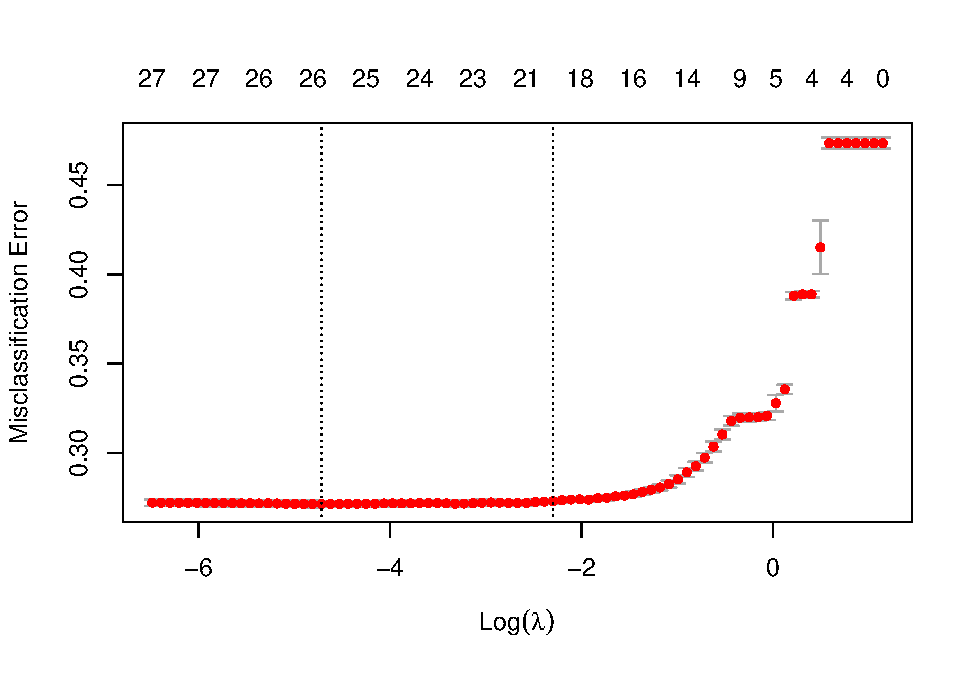
\includegraphics{figs/NET-1.pdf}

\small

\subsubsection{Comparison of Logistic
Classifiers}\label{comparison-of-logistic-classifiers}

For Logistic Regression we defined 3 Logistic classifiers. In order to
identify the best model we can compare their performance on the test
sets to see how well they captured the underlying pattern of the data
and their ability to generalize to new data.

\small

\begin{Shaded}
\begin{Highlighting}[]
\CommentTok{\# 1. Basic Logistic Classifier}
\NormalTok{glm.FULL.predict }\OtherTok{\textless{}{-}} \FunctionTok{predict}\NormalTok{(glm.FULL, }\AttributeTok{newdata =}\NormalTok{ X.test, }\AttributeTok{type =} \StringTok{"response"}\NormalTok{)}

\CommentTok{\# 2. Feature Selection with Backward Stepwise Search}
\NormalTok{glm.BACKWARD.predict }\OtherTok{\textless{}{-}} \FunctionTok{predict}\NormalTok{(glm.BACKWARD, }\AttributeTok{newdata =}\NormalTok{ X.test, }\AttributeTok{type =} \StringTok{"response"}\NormalTok{)}

\CommentTok{\# 3. Elastic Net Shrinkage Method}
\NormalTok{glm.ELNET.predict }\OtherTok{\textless{}{-}} \FunctionTok{predict}\NormalTok{(glm.ELNET, }\AttributeTok{newx =} \FunctionTok{as.matrix}\NormalTok{(X.test), }\AttributeTok{type =} \StringTok{"response"}\NormalTok{,}
    \AttributeTok{s =}\NormalTok{ best.lamda)}
\end{Highlighting}
\end{Shaded}

\small

We can use ROC curve and AUC values to compare the models. The ROC curve
is a tool for assessing the performance of binary classification models,
plotting true positive rate against false positive rate at various
thresholds. The Area Under the Curve (AUC) provides a measure of the
model's ability to predict the target values, with higher values
indicating better performance.

\small

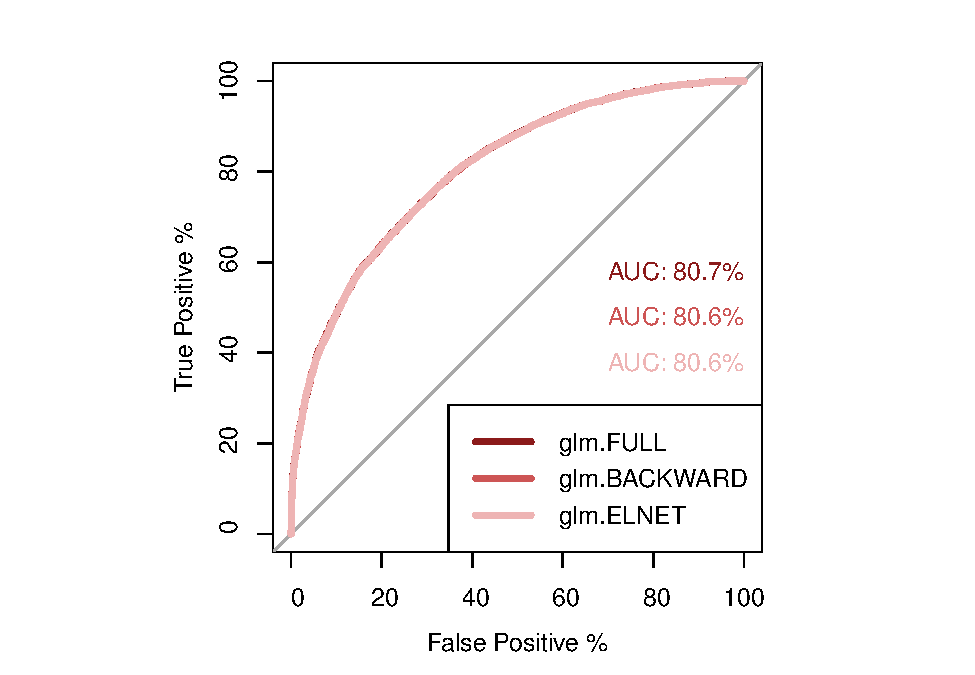
\includegraphics{figs/roc_auc-1.pdf}

\small

Although the AUC values are same, to better analyse the difference
between the model performances we can calculate and compare the
evaluation metrics.

\small

\begin{Shaded}
\begin{Highlighting}[]
\CommentTok{\# Function to evaluate prediction models at different thresholds}
\NormalTok{evaluate.model.performance }\OtherTok{\textless{}{-}} \ControlFlowTok{function}\NormalTok{(predictions, y.test, }\AttributeTok{thresholds =} \ConstantTok{NULL}\NormalTok{) \{}
\NormalTok{    output.list }\OtherTok{\textless{}{-}} \FunctionTok{list}\NormalTok{()}

    \ControlFlowTok{if}\NormalTok{ (}\SpecialCharTok{!}\FunctionTok{is.null}\NormalTok{(thresholds)) \{}
        \CommentTok{\# Looping through each threshold to generate predictions and}
        \CommentTok{\# store in output.list}
        \ControlFlowTok{for}\NormalTok{ (threshold }\ControlFlowTok{in}\NormalTok{ thresholds) \{}
\NormalTok{            output }\OtherTok{\textless{}{-}} \FunctionTok{ifelse}\NormalTok{(predictions }\SpecialCharTok{\textgreater{}}\NormalTok{ threshold, }\DecValTok{1}\NormalTok{, }\DecValTok{0}\NormalTok{)}
\NormalTok{            output.list[[}\FunctionTok{as.character}\NormalTok{(threshold)]] }\OtherTok{\textless{}{-}}\NormalTok{ output}
\NormalTok{        \}}
\NormalTok{    \} }\ControlFlowTok{else}\NormalTok{ \{}
        \CommentTok{\# Use the given predictions directly if no thresholds are}
        \CommentTok{\# provided}
\NormalTok{        output.list[[}\StringTok{"No Threshold"}\NormalTok{]] }\OtherTok{\textless{}{-}}\NormalTok{ predictions}
\NormalTok{        thresholds }\OtherTok{\textless{}{-}} \FunctionTok{c}\NormalTok{(}\StringTok{"No Threshold"}\NormalTok{)  }\CommentTok{\# Create a single \textquotesingle{}threshold\textquotesingle{} for consistent processing}
\NormalTok{    \}}

    \CommentTok{\# Initialize a data frame to store the evaluation metrics for each}
    \CommentTok{\# threshold}
\NormalTok{    results }\OtherTok{\textless{}{-}} \FunctionTok{data.frame}\NormalTok{(}\AttributeTok{Threshold =} \FunctionTok{character}\NormalTok{(}\FunctionTok{length}\NormalTok{(thresholds)), }\AttributeTok{Accuracy =} \FunctionTok{numeric}\NormalTok{(}\FunctionTok{length}\NormalTok{(thresholds)),}
        \AttributeTok{F1.Score =} \FunctionTok{numeric}\NormalTok{(}\FunctionTok{length}\NormalTok{(thresholds)), }\AttributeTok{Precision =} \FunctionTok{numeric}\NormalTok{(}\FunctionTok{length}\NormalTok{(thresholds)),}
        \AttributeTok{Recall =} \FunctionTok{numeric}\NormalTok{(}\FunctionTok{length}\NormalTok{(thresholds)))}

    \CommentTok{\# Compute evaluation metrics for each threshold}
    \ControlFlowTok{for}\NormalTok{ (i }\ControlFlowTok{in} \DecValTok{1}\SpecialCharTok{:}\FunctionTok{length}\NormalTok{(thresholds)) \{}
\NormalTok{        threshold }\OtherTok{\textless{}{-}}\NormalTok{ thresholds[i]}
\NormalTok{        predict.output }\OtherTok{\textless{}{-}}\NormalTok{ output.list[[}\FunctionTok{as.character}\NormalTok{(threshold)]]}

        \CommentTok{\# Store results in the results dataframe}
\NormalTok{        results[i, }\StringTok{"Threshold"}\NormalTok{] }\OtherTok{=}\NormalTok{ threshold}
\NormalTok{        results[i, }\StringTok{"Accuracy"}\NormalTok{] }\OtherTok{=} \FunctionTok{mean}\NormalTok{(predict.output }\SpecialCharTok{==}\NormalTok{ y.test)}
\NormalTok{        results[i, }\StringTok{"F1.Score"}\NormalTok{] }\OtherTok{=}\NormalTok{ (}\DecValTok{2} \SpecialCharTok{*} \FunctionTok{sum}\NormalTok{((predict.output }\SpecialCharTok{==} \DecValTok{1} \SpecialCharTok{\&}\NormalTok{ y.test }\SpecialCharTok{==}
            \DecValTok{1}\NormalTok{))}\SpecialCharTok{/}\NormalTok{(}\DecValTok{2} \SpecialCharTok{*} \FunctionTok{sum}\NormalTok{((predict.output }\SpecialCharTok{==} \DecValTok{1} \SpecialCharTok{\&}\NormalTok{ y.test }\SpecialCharTok{==} \DecValTok{1}\NormalTok{)) }\SpecialCharTok{+} \FunctionTok{sum}\NormalTok{(predict.output }\SpecialCharTok{==}
            \DecValTok{1} \SpecialCharTok{\&}\NormalTok{ y.test }\SpecialCharTok{==} \DecValTok{0}\NormalTok{) }\SpecialCharTok{+} \FunctionTok{sum}\NormalTok{(predict.output }\SpecialCharTok{==} \DecValTok{0} \SpecialCharTok{\&}\NormalTok{ y.test }\SpecialCharTok{==} \DecValTok{1}\NormalTok{)))}
\NormalTok{        results[i, }\StringTok{"Precision"}\NormalTok{] }\OtherTok{=} \FunctionTok{sum}\NormalTok{(predict.output }\SpecialCharTok{==} \DecValTok{1} \SpecialCharTok{\&}\NormalTok{ y.test }\SpecialCharTok{==} \DecValTok{1}\NormalTok{)}\SpecialCharTok{/}\FunctionTok{sum}\NormalTok{(predict.output }\SpecialCharTok{==}
            \DecValTok{1}\NormalTok{)}
\NormalTok{        results[i, }\StringTok{"Recall"}\NormalTok{] }\OtherTok{=} \FunctionTok{sum}\NormalTok{(predict.output }\SpecialCharTok{==} \DecValTok{1} \SpecialCharTok{\&}\NormalTok{ y.test }\SpecialCharTok{==} \DecValTok{1}\NormalTok{)}\SpecialCharTok{/}\FunctionTok{sum}\NormalTok{(y.test }\SpecialCharTok{==}
            \DecValTok{1}\NormalTok{)}
\NormalTok{    \}}

    \CommentTok{\# Rounding results}
\NormalTok{    results[, }\FunctionTok{c}\NormalTok{(}\StringTok{"Accuracy"}\NormalTok{, }\StringTok{"F1.Score"}\NormalTok{, }\StringTok{"Precision"}\NormalTok{, }\StringTok{"Recall"}\NormalTok{)] }\OtherTok{\textless{}{-}} \FunctionTok{round}\NormalTok{(results[,}
        \FunctionTok{c}\NormalTok{(}\StringTok{"Accuracy"}\NormalTok{, }\StringTok{"F1.Score"}\NormalTok{, }\StringTok{"Precision"}\NormalTok{, }\StringTok{"Recall"}\NormalTok{)], }\DecValTok{4}\NormalTok{)}

    \CommentTok{\# Conditionally adjust the output to remove the Threshold column if}
    \CommentTok{\# not needed}
    \ControlFlowTok{if}\NormalTok{ (}\FunctionTok{length}\NormalTok{(thresholds) }\SpecialCharTok{==} \DecValTok{1} \SpecialCharTok{\&\&}\NormalTok{ thresholds[}\DecValTok{1}\NormalTok{] }\SpecialCharTok{==} \StringTok{"No Threshold"}\NormalTok{) \{}
\NormalTok{        results }\OtherTok{\textless{}{-}}\NormalTok{ results[, }\SpecialCharTok{{-}}\DecValTok{1}\NormalTok{]  }\CommentTok{\# Remove the Threshold column}
        \FunctionTok{colnames}\NormalTok{(results) }\OtherTok{\textless{}{-}} \FunctionTok{c}\NormalTok{(}\StringTok{"Accuracy"}\NormalTok{, }\StringTok{"F1.Score"}\NormalTok{, }\StringTok{"Precision"}\NormalTok{, }\StringTok{"Recall"}\NormalTok{)}
        \FunctionTok{kable}\NormalTok{(results, }\AttributeTok{align =} \StringTok{"c"}\NormalTok{)}
\NormalTok{    \} }\ControlFlowTok{else}\NormalTok{ \{}
        \FunctionTok{kable}\NormalTok{(results, }\AttributeTok{align =} \StringTok{"c"}\NormalTok{)}
\NormalTok{    \}}
\NormalTok{\}}
\end{Highlighting}
\end{Shaded}

\small

\small

\begin{Shaded}
\begin{Highlighting}[]
\NormalTok{thresholds }\OtherTok{\textless{}{-}} \FunctionTok{c}\NormalTok{(}\FloatTok{0.2}\NormalTok{, }\FloatTok{0.3}\NormalTok{, }\FloatTok{0.4}\NormalTok{, }\FloatTok{0.5}\NormalTok{, }\FloatTok{0.6}\NormalTok{)}

\CommentTok{\# 1. Basic Logistic Classifier}
\FunctionTok{evaluate.model.performance}\NormalTok{(glm.FULL.predict, y.test, thresholds)}
\end{Highlighting}
\end{Shaded}

\begin{longtable}[]{@{}ccccc@{}}
\toprule\noalign{}
Threshold & Accuracy & F1.Score & Precision & Recall \\
\midrule\noalign{}
\endhead
\bottomrule\noalign{}
\endlastfoot
0.2 & 0.6401 & 0.7367 & 0.5941 & 0.9692 \\
0.3 & 0.6912 & 0.7554 & 0.6417 & 0.9179 \\
0.4 & 0.7215 & 0.7593 & 0.6889 & 0.8456 \\
0.5 & 0.7313 & 0.7456 & 0.7337 & 0.7578 \\
0.6 & 0.7263 & 0.7120 & 0.7850 & 0.6515 \\
\end{longtable}

\begin{Shaded}
\begin{Highlighting}[]
\CommentTok{\# 2. Feature Selection with Backward Stepwise Search}
\FunctionTok{evaluate.model.performance}\NormalTok{(glm.BACKWARD.predict, y.test, thresholds)}
\end{Highlighting}
\end{Shaded}

\begin{longtable}[]{@{}ccccc@{}}
\toprule\noalign{}
Threshold & Accuracy & F1.Score & Precision & Recall \\
\midrule\noalign{}
\endhead
\bottomrule\noalign{}
\endlastfoot
0.2 & 0.6395 & 0.7363 & 0.5937 & 0.9691 \\
0.3 & 0.6907 & 0.7549 & 0.6414 & 0.9170 \\
0.4 & 0.7226 & 0.7601 & 0.6901 & 0.8458 \\
0.5 & 0.7323 & 0.7467 & 0.7343 & 0.7595 \\
0.6 & 0.7270 & 0.7129 & 0.7855 & 0.6525 \\
\end{longtable}

\begin{Shaded}
\begin{Highlighting}[]
\CommentTok{\# 3. Elastic Net Shrinkage Method}
\FunctionTok{evaluate.model.performance}\NormalTok{(glm.ELNET.predict, y.test, thresholds)}
\end{Highlighting}
\end{Shaded}

\begin{longtable}[]{@{}ccccc@{}}
\toprule\noalign{}
Threshold & Accuracy & F1.Score & Precision & Recall \\
\midrule\noalign{}
\endhead
\bottomrule\noalign{}
\endlastfoot
0.2 & 0.6266 & 0.7306 & 0.5842 & 0.9748 \\
0.3 & 0.6829 & 0.7524 & 0.6328 & 0.9278 \\
0.4 & 0.7214 & 0.7609 & 0.6864 & 0.8536 \\
0.5 & 0.7316 & 0.7462 & 0.7332 & 0.7598 \\
0.6 & 0.7247 & 0.7083 & 0.7876 & 0.6435 \\
\end{longtable}

\small

All of the models have the highest F1 score at threshold level 0.4. And
F1 score with 0.4 threshold for glm.ELNET is higher than other models on
the test set. These results indicate that the model with Elastic Net
regularization is better in generalization. Therefore we can select the
glm.ELNET.predict as the best prediction for logistic regression model.

\subsection{LDA \& QDA}\label{lda-qda}

Linear Discriminant Analysis (LDA) is a classification algorithm that
finds a linear combination of features that best separates two or more
classes. It assumes that the features follow a multivariate normal
distribution with a common mean and variance for all classes. LDA and
logistic classifier have the same (linear) form but LDA makes more
assumptions about the underlying data then the logistic classifier. For
the model we decided to exclude the features that had high VIF and
p-values as analysed for logistic classifiers.

\small

\begin{Shaded}
\begin{Highlighting}[]
\CommentTok{\# Perform LDA modelling on train data and make predictions on test data}
\NormalTok{lda.model }\OtherTok{\textless{}{-}} \FunctionTok{lda}\NormalTok{(AttritionStayed }\SpecialCharTok{\textasciitilde{}}\NormalTok{ . }\SpecialCharTok{{-}}\NormalTok{ Job.RoleFinance }\SpecialCharTok{{-}}\NormalTok{ Job.RoleTechnology }\SpecialCharTok{{-}}
\NormalTok{    Job.RoleHealthcare }\SpecialCharTok{{-}}\NormalTok{ Monthly.Income }\SpecialCharTok{{-}}\NormalTok{ Education.LevelBachelor.s.Degree }\SpecialCharTok{{-}}
\NormalTok{    Education.LevelHigh.School }\SpecialCharTok{{-}}\NormalTok{ Education.LevelMaster.s.Degree }\SpecialCharTok{{-}}\NormalTok{ Employee.Recognition,}
    \AttributeTok{data =}\NormalTok{ train.data)}
\NormalTok{lda.model}
\end{Highlighting}
\end{Shaded}

\begin{verbatim}
Call:
lda(AttritionStayed ~ . - Job.RoleFinance - Job.RoleTechnology - 
    Job.RoleHealthcare - Monthly.Income - Education.LevelBachelor.s.Degree - 
    Education.LevelHigh.School - Education.LevelMaster.s.Degree - 
    Employee.Recognition, data = train.data)

Prior probabilities of groups:
        0         1 
0.4733213 0.5266787 

Group means:
        Age GenderMale Years.at.Company Job.RoleMedia Work.Life.Balance
0 0.4852905   0.497359        0.2793094     0.1595590         0.5121888
1 0.5144369   0.595782        0.3085520     0.1630189         0.4743169
  Job.Satisfaction Performance.Rating Number.of.Promotions OvertimeYes
0        0.3880795          0.2453354            0.1869616   0.3535397
1        0.3474890          0.2227213            0.2273886   0.3008697
  Distance.from.Home Education.LevelPhD Marital.StatusMarried
0          0.5287533         0.02552377             0.3808359
1          0.4736951         0.07359266             0.6108828
  Marital.StatusSingle Number.of.Dependents Job.Level Company.Size
0            0.4904818            0.2545287 0.2765252    0.5579071
1            0.2220205            0.2943335 0.5128548    0.5430246
  Remote.WorkYes Leadership.OpportunitiesYes Innovation.OpportunitiesYes
0     0.09901095                  0.04707717                   0.1548087
1     0.27130523                  0.05234318                   0.1699959
  Company.Reputation
0          0.6126768
1          0.5927979

Coefficients of linear discriminants:
                                    LD1
Age                          0.17822014
GenderMale                   0.42558074
Years.at.Company             0.50701891
Job.RoleMedia                0.03304174
Work.Life.Balance           -0.44238318
Job.Satisfaction            -0.28451537
Performance.Rating          -0.22952580
Number.of.Promotions         0.72414409
OvertimeYes                 -0.26331157
Distance.from.Home          -0.69131133
Education.LevelPhD           1.10625973
Marital.StatusMarried        0.20731266
Marital.StatusSingle        -1.14089514
Number.of.Dependents         0.65669259
Job.Level                    1.83688216
Company.Size                -0.15697901
Remote.WorkYes               1.23658524
Leadership.OpportunitiesYes  0.12997879
Innovation.OpportunitiesYes  0.09931127
Company.Reputation          -0.26718594
\end{verbatim}

\begin{Shaded}
\begin{Highlighting}[]
\NormalTok{lda.predict }\OtherTok{\textless{}{-}} \FunctionTok{predict}\NormalTok{(lda.model, }\AttributeTok{newdata =}\NormalTok{ test.data)}\SpecialCharTok{$}\NormalTok{class}

\CommentTok{\# Evaluate the performance of the model}
\FunctionTok{evaluate.model.performance}\NormalTok{(lda.predict, y.test)}
\end{Highlighting}
\end{Shaded}

\begin{longtable}[]{@{}cccc@{}}
\toprule\noalign{}
Accuracy & F1.Score & Precision & Recall \\
\midrule\noalign{}
\endhead
\bottomrule\noalign{}
\endlastfoot
0.7336 & 0.7471 & 0.7368 & 0.7576 \\
\end{longtable}

\small

Quadratic Discriminant Analysis (QDA) is similar to LDA but allows for
different mean and variance for each class. This results in quadratic
decision boundaries.

\small

\begin{Shaded}
\begin{Highlighting}[]
\NormalTok{qda.model }\OtherTok{\textless{}{-}} \FunctionTok{qda}\NormalTok{(AttritionStayed }\SpecialCharTok{\textasciitilde{}}\NormalTok{ . }\SpecialCharTok{{-}}\NormalTok{ Job.RoleFinance }\SpecialCharTok{{-}}\NormalTok{ Job.RoleTechnology }\SpecialCharTok{{-}}
\NormalTok{    Job.RoleHealthcare }\SpecialCharTok{{-}}\NormalTok{ Monthly.Income }\SpecialCharTok{{-}}\NormalTok{ Education.LevelBachelor.s.Degree }\SpecialCharTok{{-}}
\NormalTok{    Education.LevelHigh.School }\SpecialCharTok{{-}}\NormalTok{ Education.LevelMaster.s.Degree }\SpecialCharTok{{-}}\NormalTok{ Employee.Recognition,}
    \AttributeTok{data =}\NormalTok{ train.data)}
\NormalTok{qda.predict }\OtherTok{\textless{}{-}} \FunctionTok{predict}\NormalTok{(qda.model, }\AttributeTok{newdata =}\NormalTok{ test.data)}\SpecialCharTok{$}\NormalTok{class}
\NormalTok{qda.model}
\end{Highlighting}
\end{Shaded}

\begin{verbatim}
Call:
qda(AttritionStayed ~ . - Job.RoleFinance - Job.RoleTechnology - 
    Job.RoleHealthcare - Monthly.Income - Education.LevelBachelor.s.Degree - 
    Education.LevelHigh.School - Education.LevelMaster.s.Degree - 
    Employee.Recognition, data = train.data)

Prior probabilities of groups:
        0         1 
0.4733213 0.5266787 

Group means:
        Age GenderMale Years.at.Company Job.RoleMedia Work.Life.Balance
0 0.4852905   0.497359        0.2793094     0.1595590         0.5121888
1 0.5144369   0.595782        0.3085520     0.1630189         0.4743169
  Job.Satisfaction Performance.Rating Number.of.Promotions OvertimeYes
0        0.3880795          0.2453354            0.1869616   0.3535397
1        0.3474890          0.2227213            0.2273886   0.3008697
  Distance.from.Home Education.LevelPhD Marital.StatusMarried
0          0.5287533         0.02552377             0.3808359
1          0.4736951         0.07359266             0.6108828
  Marital.StatusSingle Number.of.Dependents Job.Level Company.Size
0            0.4904818            0.2545287 0.2765252    0.5579071
1            0.2220205            0.2943335 0.5128548    0.5430246
  Remote.WorkYes Leadership.OpportunitiesYes Innovation.OpportunitiesYes
0     0.09901095                  0.04707717                   0.1548087
1     0.27130523                  0.05234318                   0.1699959
  Company.Reputation
0          0.6126768
1          0.5927979
\end{verbatim}

\begin{Shaded}
\begin{Highlighting}[]
\FunctionTok{evaluate.model.performance}\NormalTok{(qda.predict, y.test)}
\end{Highlighting}
\end{Shaded}

\begin{longtable}[]{@{}cccc@{}}
\toprule\noalign{}
Accuracy & F1.Score & Precision & Recall \\
\midrule\noalign{}
\endhead
\bottomrule\noalign{}
\endlastfoot
0.713 & 0.6968 & 0.7718 & 0.6351 \\
\end{longtable}

\small

\end{document}
